% !TEX root = ../main_lecture_notes.tex
\chapter{Security of blockchain systems}\label{chap:security}
The security evaluation of blockchain systems consists of calculating the probability of a successful attack on the blockchain. We will focus on the double spending attack. \cref{sec:double_spending} provides a brief overview through a simple example. The probability of a successful double spending attack is computed within a random walk model in \cref{sec:double_spending_rw} and counting processes in \cref{sec:counting_process}.

\section{Double-spending in PoW}\label{sec:double_spending}
A double spending attack aims to generate a concurrent blockchain to replace the main one. Consider the following scenario:

\begin{enumerate}
\item Marie sends BTC$10$ to John.
\item The transaction from Marie to John is recorded in the blockchain.
\item John is advised to wait for $\alpha$ confirmations, meaning $\alpha-1$ blocks need to be appended after the block where the Marie to John transaction is recorded.
\item Once $\alpha$ confirmations have been received, John ships the goods.
\item Meanwhile, Marie has started working on her own blockchain version where the Marie to John transaction is replaced by a Marie to Marie transaction.
\item At the shipment date, the main blockchain is ahead by $xx$ blocks.
\item Marie's goal is then to work on her blockchain branch to catch up with the main branch. If she manages to do that, her branch will replace the public branch, and she will recover her bitcoin. She can therefore spend these bitcoins again, hence the name double spending.
\end{enumerate}
The race between the two competing branches of the blockchain is summarized on \cref{fig:dp_illustration}.
\begin{figure}[ht!]
\begin{center}
\begin{tikzpicture}[-, >=stealth', auto, semithick, node distance=1cm]
% \tikzstyle{block} = [rectangle, draw, fill=blue!20,
%     text width=5em, text centered, rounded corners]
\tikzstyle{block}=[rectangle, fill=black,draw=black,thick,text=black,scale=1.5]
\tikzstyle{block}=[rectangle, fill=white,draw=black,thick,text=black,scale=1.5]
\tikzstyle{confirmed block}=[rectangle, fill=white,draw=blue,thick,text=black,scale=1.5]
\tikzstyle{bad block}=[rectangle, fill=white,draw=red,thick,text=black,scale=1.5]
\node[block]    (1)                     {\tiny $\text{M}\rightarrow \text{J}$};
\node[block]    (2)[right of=1]                     {};
\node[block]    (3)[right of=2]                     {};
\node[block]    (4)[right of=3]                     {};
\node[confirmed block]    (5)[right of=4]                     {};

\node[bad block]    (6)[below of=1]         {\tiny $\text{M}\rightarrow \text{M}$};
\node[block]    (7)[right of=6]         {};
\node[block]    (8)[right of=7]         {};
\path
(1) edge[ left]     node{}     (2)
(2) edge[ left]     node{}     (3)
(3) edge[ left]     node{}     (4)
(4) edge[ left]     node{}     (5)
(6) edge[ left]     node{}     (7)
(7) edge[ left]     node{}     (8);

\end{tikzpicture}
\end{center}
\caption{Double spending race illustrated, here we have $\alpha = 4$ and $X = 2$.}
\label{fig:dp_illustration}
\end{figure}
\section{Random walk model}\label{sec:double_spending_rw}
We define a discrete-time stochastic process $(X_n)_{n\geq0}$ as the difference in length between the public and the private branches of the blockchain. At each time step, when a block is found, it belongs to the main branch with probability $p$ and to the other branch with probability $q=1-p$. Here, the parameter $p$ represents the proportion of hashpower owned by the honest miners, while $q$ represents that of the attacker. We have
$$
X_0 = X\text{, and  }X_n = x+\xi_1+\ldots+ \xi_n.
$$
The $\xi_i$'s are \iid random variables such that 
$$
\mathbb{P}(\xi=1) = p\in (0,1)\text{, and }\mathbb{P}(\xi=-1) = 1-p=q,
$$ 
$(X_n)_{n\geq0}$ is therefore a random walk on $\mathbb{Z}$. We assume that $p>q$ so that the attacker does not hold more than half of the total hashpower. Define the double spending time as 
$$
{\tau_0} = \inf\{n>0\text{ ; }X_n = 0\}.
$$
Our goal is to study the distribution of this stopping time with respect to the filtration 
$$
\mathcal{F}_n = \sigma(\xi_1,\ldots, \xi_n),\text{ }n\geq1.
$$ 
An illustration of this first-hitting time problem is provided in \cref{fig:double_spending_time}.
\begin{figure}[ht!]
\begin{center}
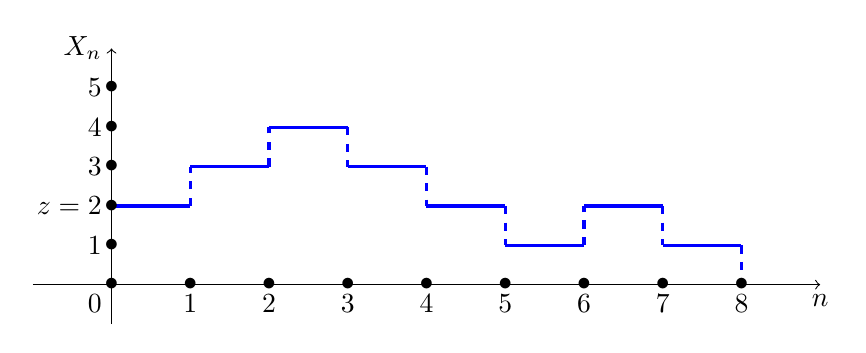
\begin{tikzpicture}
  %Origin and axis
  \coordinate (O) at (0,0);
  \draw[->] (-1,0) -- (9,0) coordinate[label = {below:$n$}] (xmax);
  \draw[->] (0,-0.5) -- (0,3) coordinate[label = {left:$X_n$}] (ymax);
  %Lower linear boundary

 
  %Stochastic process trajectory
  
  \draw (0,0) node[blue,left] {} node{};
  \draw[very thick,blue,-] (0,1) -- (1,1) node[pos=0.5, above] {} ;
  \draw[very thick,dashed,blue] (1,1) -- (1,1.5) node[pos=0.5, right] {};
  \draw[very thick,blue,-] (1,1.5) -- (2,1.5) node[pos=0.5, above] {};
  \draw[very thick,dashed,blue] (2,1.5) -- (2,2) node[pos=0.5, right] {};
  \draw[very thick,blue,-] (2,2) -- (3,2) node[pos=0.5, above] {};
  \draw[very thick,dashed,blue] (3,2) -- (3,1.5) node[pos=0.5, right] {};
  \draw[very thick,blue,-] (3,1.5) -- (4,1.5)node[pos=0.5, above] {};
  \draw[very thick,dashed,blue] (4,1.5) -- (4,1) node[pos=0.5, right] {};  
  \draw[very thick,blue,-] (4,1) -- (5,1) node[pos=0.5, above] {};
  \draw[very thick,dashed,blue] (5,1) -- (5,0.5) node[pos=0.5, right] {};  
  \draw[very thick,blue,-] (5,0.5) -- (6,0.5) node[pos=0.5, above] {};
  \draw[very thick,dashed,blue,-] (6,0.5) -- (6,1) node[pos=0.5, above] {};
   \draw[very thick,blue,-] (6,1) -- (7,1) node[pos=0.5, above] {};
    \draw[very thick,dashed,blue,-] (7,1) -- (7,0.5) node[pos=0.5, above] {};
     \draw[very thick,blue,-] (7,0.5) -- (8,0.5) node[pos=0.5, above] {};
     \draw[very thick,dashed,blue,-] (8,0.5) -- (8,0) node[pos=0.5, above] {};
  %Jump Times
  \draw (1,0) node[black,below] {$1$} node{ \color{black}$\bullet$};
  \draw (2,0) node[black,below] {$2$} node{ \color{black}$\bullet$};
  \draw (3,0) node[black,below] {$3$} node{ \color{black}$\bullet$};
  \draw (4,0) node[black,below] {$4$} node{ \color{black}$\bullet$};
  \draw (5,0) node[black,below] {$5$} node{ \color{black}$\bullet$};
  \draw (6,0) node[black,below] {$6$} node{ \color{black}$\bullet$};
  \draw (7,0) node[black,below] {$7$} node{ \color{black}$\bullet$};
  \draw (8,0) node[black,below] {$8$} node{ \color{black}$\bullet$};
  %Level of the counting process
   \draw (0,0) node[black,below left] {$0$} node{ \color{black}$\bullet$};
   \draw (0,0.5) node[black,left] {$1$} node{ \color{black}$\bullet$};
   \draw (0,1) node[black,left] {$z=2$} node{ \color{black}$\bullet$};
   \draw (0,1.5) node[black,left] {$3$} node{ \color{black}$\bullet$};
   \draw (0,2) node[black,left] {$4$} node{ \color{black}$\bullet$};
   \draw (0,2.5) node[black,left] {$5$} node{ \color{black}$\bullet$};

  % %Aggregated Capital gains
%  \draw (0,1.5) node[blue,below right] {$\mu_1$} node{ \color{blue}$-$};
%  \draw (0,2.25) node[blue,left] {$\mu_2$} node{ \color{blue}$-$};
%  \draw (0,3.75) node[blue,left] {$\mu_3$} node{ \color{blue}$-$};
  %Ruin time = First-crossing time time
%  \draw (5,0) node[black,above right] {${\tau_0}_u$} node{ \color{black}$\times$};
%  \draw[dotted,black] (0,3.28) -- (5,3.28);
%  \draw[dotted,black] (5,0) -- (5,3.28);
\end{tikzpicture}
\end{center}
\caption{Illustration of the first-hitting time problem of a double spending attack.}
\label{fig:double_spending_time}
\end{figure}
Let us denote by 
$$
\mathbb{P}_x(\cdot) = \mathbb{P}(\cdot|X_0 = x)\text{ and }\mathbb{E}_x(\cdot) = \mathbb{E}(\cdot|X_0 = x) 
$$
We are interested for now in the conditional distribution of ${\tau_0}$ provided that $X_0 = x\geq 0$.
\subsection{Double spending probability}\label{ssec:double_spending_rw_dsp}
The double spending probability is defined as $\mathbb{P}_x({\tau_0} <\infty)$. We can compute this probability by solving the so-called gambler's ruin problem. Let $a\geq x$ and define 
$$
\tau_a = \inf\{n\geq 0\text{ ; }X_n = a\}.
$$
Further denote by 
$$
\phi(x,a) = \mathbb{P}(\tau_0 <\tau_a).
$$
Note that 
$$
\mathbb{P}_x({\tau_0} <\infty) = \underset{a\rightarrow \infty}{\lim} \phi(x,a).
$$
We have the following result
\begin{theo}
\begin{equation}\label{eq:gambler_ruin}
\phi(x,a) = \begin{cases}
\frac{(q/p)^x-(q/p)^a}{1 - (q/p)^a}&\text{ if }p\neq q,\\
\frac{a-x}{a}&\text{ if }p= q.
\end{cases}
\end{equation}
\end{theo}
\noindent We give two proofs for this result, the first one uses simple first step analysis exploiting the Markov property of the random walk. The second one uses Martingale and the optional stopping theorem.\\

\underline{\textit Proof 1:}\\
By the law of total probability, we have 
\begin{equation}\label{eq:difference_equation}
\phi(x,a) = p\phi(x,a+1)+(1-p)\phi(x,a-1),\text{ }x\geq1.
\end{equation}
We also have the boundary conditions
\begin{equation}\label{eq:boundary_conditions_double_spending}
\phi(0,a) = 1\text{ and }\phi(a,a) = 0.
\end{equation}
Equation \eqref{eq:difference_equation} is a linear difference equation of order $2$\footnote{For details about such equation on ecan check for instance \url{https://mjo.osborne.economics.utoronto.ca/index.php/tutorial/index/1/sod/t}} associated to the following characteristic equation
\begin{equation}\label{eq:characteristic_equation}
px^2 - x + 1-p = 0
\end{equation}
\begin{enumerate}

\item Assume that $p=1-p=1/2$ then \eqref{eq:characteristic_equation} has one solution 
$$
r = 1
$$
The solutions of \eqref{eq:difference_equation} are given by 
$$
\phi(x,a) = A+Bx
$$
Using the boudary conditions \eqref{eq:boundary_conditions_double_spending}, we deduce that
$$
\phi(x,a) = \frac{a-x}{a},
$$
as announced.
\item Assume that $p\neq 1-p$
which has two roots on the real line with 
$$
r_1 = 1, \text{ and }r_2 = \frac{1-p}{p}.
$$
The solution of \eqref{eq:difference_equation} is given by 
$$
\phi(x,a)=A+B\left(\frac{1-p}{p}\right)^xx,
$$
where $A$ and $B$ are constant. Using the boudary conditions \eqref{eq:boundary_conditions_double_spending}, we deduce that
$$
\phi(x,a) = \frac{(q/p)^x-(q/p)^a}{1 - (q/p)^a},
$$
as announced.
\end{enumerate}
For the second proof we need the notion of martingale
\begin{definition}
A stochastic process $(X_n)_{n\geq0}$, is called a martingale with respect to a filtration $\mathcal{F}_n$, if
\begin{itemize}
  \item[(i)] $X_n$ is $\mathcal{F}_n$-adapted
  \item[(ii)] $\mathbb{E}(X_n)<\infty\text{ for }n\geq0$ 
  \item[(iii)] $\mathbb{E}(X_n|\mathcal{F}_{n-1}) = X_{n-1}$
\end{itemize} 
\end{definition}
\noindent and the optional stopping theorem.
\begin{theo}
Let $T$ be a bounded stopping time for the martingale $(X_n)_{n\geq0}$ then it holds that 
$$
\mathbb{E}(X_T) = \mathbb{E}(X_0) .
$$
% in each of the following situations
% \begin{itemize}
% \item[(i)] $T$ is bounded almost surely 
% \item[(ii)] There exists $c>0$ such that $|X_{T\land n}|<c$ for every $n>0$.
% \item[(iii)] $\mathbb{E}(T)<\infty$, and, for some $K>0$ we have that 
% $$
% |X_n(\omega) - X_{n-1}(\omega)|\leq K,\text{ }\forall (n,\omega).
% $$
% \end{itemize}

\end{theo}
\underline{\textit Proof 2:}\\
Let $T = \tau_0\land\tau_a$, it is a bounded stopping time.\\

Assume that $p=1- p =1/2$ then $(X_n)_{n\geq 0}$ is a martingale. We apply the optionnal stopping time theorem at $T$ on $(X_n)_{n\geq 0}$. We have 
$$
\mathbb{E}(X_0) = x
$$
on one hand and 
\begin{eqnarray*}
\mathbb{E}(X_T)&=&\mathbb{E}(X_{\tau_0}\mathbb{I}_{\tau_0\leq \tau_a} + X_{\tau_a}\mathbb{I}_{\tau_0> \tau_a})\\
&=&a\mathbb{P}(\tau_0>\tau_a)\\
&=&a\left[1-\phi(x,a)\right].
\end{eqnarray*}
From $\mathbb{E}(X_0) =\mathbb{E}(X_T)$, we deduce that 
$$
\phi(x,a) = \frac{a-x}{a}.
$$
Assume that $p\neq 1-p $. Define the process 
$$
M_n^\theta = \exp\left[\theta X_n- n\kappa_\xi(\theta)\right],\text{ for }n\in\mathbb{N}\text{ and }\theta\in\mathbb{R}, 
$$
where
$$
\kappa_\xi(\theta) = \log\left[\mathbb{E}\left(e^{\theta\xi}\right)\right],
$$
is the cumulant generating function of $\xi$. 
\begin{lemma}\label{lem:wald_martingale_RW}
Take $s$ so that $\kappa_\xi(\theta)<\infty$ then $(M_n^\theta)_{n\geq0}$ is a $\mathcal{F}_n$-martingale.
\end{lemma}
\begin{proof}
We have that 
\begin{eqnarray*}
\mathbb{E}(M_n^\theta|\mathcal{F}_n)&=&\mathbb{E}\left\{\exp\left[\theta X_n - n\kappa_\xi(\theta)\right]|\mathcal{F}_{n-1}\right\}\\
&=&\exp\left[\theta X_{n-1} - n\kappa_\xi(\theta)\right]\mathbb{E}\left[\exp\left(s\xi_{n}\right)|\mathcal{F}_{n-1}\right]\\
&=&\exp\left[\theta X_{n-1}- n\kappa_\xi(\theta) \right]\exp[ \kappa_\xi(\theta) ]\\
&=& M_{n-1}.
\end{eqnarray*}
\end{proof} 
The equation $\kappa_\xi(\theta) = 0$ is equivalent to 
$$
pe^s+qe^{-s} = 1,
$$
which admits $\gamma =\log(q/p)$ as only non-zero solution. The process $(\e^{\gamma X_n})_{n\geq0}$ is a $\mathcal{F}_n$-Martingale. Define $\tau_a = \inf\{n\geq 0\text{ ; }X_n = a\}$, for $a>z$. We apply the optionnal stopping time theorem at $T$ on $\left(e^{\gamma X_n}\right)_{n\geq 0}$. We have
$$
\mathbb{E}_x(e^{\gamma X_0}) = e^{\gamma x},
$$
and 
\begin{eqnarray*}
 \mathbb{E}_x(e^{\gamma X_{T}}) &=& \mathbb{E}_x(e^{\gamma X_{\tau_0}}\mathbb{I}_{\tau_0\leq \tau_a} + e^{\gamma X_{\tau_a}}\mathbb{I}_{\tau_0> \tau_a})\\
 &=& \phi(x,a) + e^{\gamma a}(1-\phi(x,a)).
\end{eqnarray*}
From $\mathbb{E}_x(X_0) =\mathbb{E}_x(X_T)$, we deduce that 
$$
\phi(x,a) = \frac{e^{\gamma x} - e^{\gamma a}}{1- e^{\gamma a}}.
$$
which is equivalent to \eqref{eq:gambler_ruin} (recall that $\gamma =\log(q/p)$). 
\begin{coro}
Assume that $p>q$ then the double spending probability is given by 
$$
\mathbb{P}_x(\tau_0 <\infty) =\left(\frac{q}{p}\right)^x.
$$
\end{coro}
\begin{proof}
We have
$$
\mathbb{P}(\tau_0 <\infty) = \underset{a\rightarrow \infty}{\lim}\phi(x,a) = \left(\frac{q}{p}\right)^x.
$$
\end{proof}

% \begin{exercise}
% Just for fun
% \begin{itemize}
% \item What is $\phi(z)$ when $p \leq q$ ? 
% \item Compute $\mathbb{P}(\tau_0 \leq \tau_a)$ if $p = q = 1/2$
% \end{itemize}
% \end{exercise}
In practice the number of blocks $x$ is actually random variable 
$$
X = (\alpha -M)_+,
$$ 
where $M$ corresponds to the number of blocks the attacker managed to mine while the vendor waits for $\alpha$ confirmations. If we assume that a block mined by the honest miners is a success while a block mined by the attacker is a failure then $M$ actually counts the number of failure before $\alpha$ successes. We have that $M\sim \text{Neg-Bin}(\alpha, p)$ where $M$ has a probability mass function (\pmf) given by 
$$
\mathbb{P}(M = m) = \binom{\alpha+m-1}{m}p^\alpha q^m.
$$
Whenever $X = 0$ then double spending occurs right away as $\phi(0) =1$. To derive the double spending probability, we condition upon the values of $X$ via the law of total probability as
$$
\mathbb{P}( \text{Double Spending}) = \mathbb{P}(M\geq \alpha)+\sum_{m = 0}^{\alpha-1}\binom{\alpha+m-1}{m}q^\alpha p^m.
$$
The analysis conducted here is similar to that of \citet{rosenfeld2014analysis}.
\subsection{Double spending time}\label{sssec:double_spending_rw_dst}
In the block mining world, time is money. Every hour spent computing hashes is costly in terms of energy. It is therefore very interesting to know whether a double-spending attack is meant to last long or not. Intuitively, we can think that if it must occur, it should happen at an earlier stage because, as $p > 1/2$, our random walk $(X_n)_{n\geq0}$ will eventually drift towards $+\infty$. The following result provides the probability distribution of $\tau_0$ when $X_0 = x$.
\begin{theo}
If $x = 0$ then $\tau_0=0$ almost surely. If $x>0$ then $\tau_0$ admits a \pmf given by 
$$
\mathbb{P}_x(\tau_0 = n)=
\frac{x}{n}\binom{n}{(n-x) / 2}p^{(n-x) / 2}q^{(n
+x) / 2}\text{ if }n\geq x\text{ and }n-x\text{ is even},
$$
and $0$ otherwise.
\end{theo}
\begin{proof}
We start by showing the following lemma, sometimes referred to as the Markov hitting time theorem.
\begin{lemma}\label{lem:markov_hitting_time}
\begin{equation}\label{eq:markov_hitting_time}
\mathbb{P}_x(\tau_0 = n) = \frac{x}{n}\mathbb{P}_x(X_n = 0),\text{ }x\geq 0,\text{ and }n> 0.
\end{equation}
\end{lemma}
\begin{proof}
If $x = 0$ then $\tau_0 = 0$ almost surely and both sides of \eqref{eq:markov_hitting_time} equal to $0$. Assume that $x\geq1$, we have that $\mathbb{P}_x(\tau_0 = n) = 0$ and $\mathbb{P}_x(X_n = 0) = 0$ whenever $n<x$ or $n-x$ is odd. The rest of the proof is by induction on $n\geq1$, when $n = 1$ we have that 
$$
\mathbb{P}_x(\tau_0 = 1) = 0 = \frac{x}{1}\mathbb{P}_x(X_1 = 0),\text{ for }x>1, 
$$
and 
$$\mathbb{P}_1(\tau_0 = 1) = q = \frac{1}{1}\mathbb{P}_1(X_1 = 0),\text{ for }x=1. 
$$
The property holds for $n=1$. Assume that it holds for some $n\geq1$. The law of total probability yields
\begin{eqnarray*}
\mathbb{P}_x(\tau_0 = n+1)&=&\sum_{y\in\{-1,1\}}\mathbb{P}_x(\tau_0 = n+1|\xi_1 = y)\mathbb{P}(\xi_1 = y)\\
&=&\sum_{y\in\{-1,1\}}\mathbb{P}_{x+y}(\tau_0 = n)\mathbb{P}(\xi_1 = y) \text{ (Strong Markov Property)}\\
&=&\sum_{y\in\{-1,1\}}\frac{x+y}{n}\mathbb{P}_{x+y}(X_n = 0)\mathbb{P}(\xi_1 = y).
\end{eqnarray*}
 Note that for any measurable application $g$ we have
\begin{eqnarray*}
\mathbb{E}_x[g(\xi_1)\mathbb{I}_{X_{n+1}=0}]&=&\sum_{y\in\{-1,1\}}\mathbb{E}_x[g(\xi_1)\mathbb{I}_{X_{n+1}=0}|\xi_1 = y]\mathbb{P}(\xi_1=y)\\
&=&\sum_{y\in\{-1,1\}}g(y)\mathbb{P}_x(X_{n+1}=0|\xi_1 = y)\mathbb{P}(\xi_1=y)\\
&=&\sum_{y\in\{-1,1\}}g(y)\mathbb{P}_{x+y}(X_{n}=0)\mathbb{P}(\xi_1=y)
\end{eqnarray*}
Take $g(y) = \frac{x+y}{n}$ and further undo the law of total probability, 
\begin{eqnarray}
\mathbb{P}_x(\tau_0 = n+1)&=&\sum_{y\in\{-1,1\}}\frac{x+y}{n}\mathbb{P}_{x+y}(X_n = 0)\mathbb{P}(\xi_1 = y)\nonumber\\
&=&\sum_{y\in\{-1,1\}}\frac{x+y}{n}\mathbb{P}_{x}(X_{n+1} = 0|\xi_1 = y)\mathbb{P}(\xi_1 = y)\nonumber\\
&=&\sum_{y\in\{-1,1\}}\frac{x+y}{n}\mathbb{P}_{x}(\xi_1 = y|X_{n+1} = 0)\mathbb{P}_x(X_{n+1} = 0)\nonumber\\
&=&\frac{\mathbb{P}_x(X_{n+1} = 0)}{n}\left[x+\mathbb{E}(\xi_1|X_{n+1}=0)\right].\label{eq:law_total_probability_undone}
\end{eqnarray}
Since the $\xi_i$ are \iid then it holds that 
$$
\mathbb{E}(\xi_1|X_{n+1}=0) = \mathbb{E}(\xi_i|X_{n+1}=0)\text{, } i = 1, \ldots, n+1,
$$
and it follows that 
$$
\mathbb{E}(\xi_1|X_{n+1}=0) = \frac{1}{n+1}\sum_{i =1}^{n+1}\mathbb{E}(\xi_i|X_{n+1}=0) = \frac{-x}{n+1}.
$$
Inserting the above expression in \eqref{eq:law_total_probability_undone} yields 
$$
\mathbb{P}_x(\tau_0 = n+1) = \frac{x}{n+1}\mathbb{P}_x(X_{n+1} = 0).
$$
\end{proof}
\begin{remark}
This proof is direct, simple and inspired from \citet{Hofstad2008}. It is possible to make it shorter by taking advantage of the ballot theorem. Indeed, consider again the first hitting problem on \cref{fig:double_spending_time} and reverse the timeline. It corresponds to that of a random walk $(S_n)_{n\geq0}$ that starts at $0$, make upward jumps with probability $q$, and ends up at the level $x$ at time $n$ without crossing the $X$ axis, see \cref{fig:time_reversed_double_spending_time}.
\begin{figure}[ht!]
\begin{center}
 \subfloat[Original first hitting problem]
 {
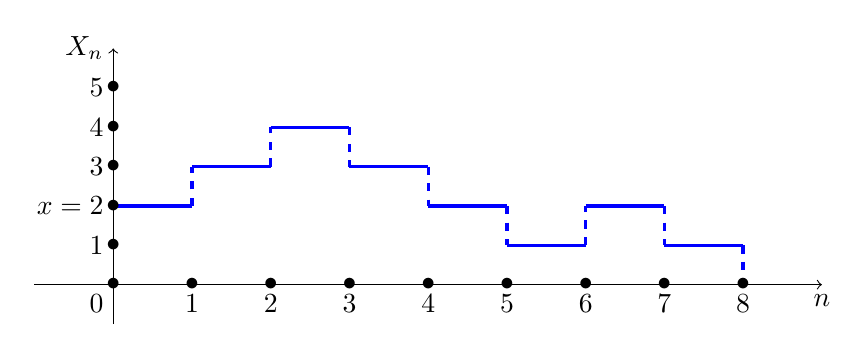
\begin{tikzpicture}
  %Origin and axis
  \coordinate (O) at (0,0);
  \draw[->] (-1,0) -- (9,0) coordinate[label = {below:$n$}] (xmax);
  \draw[->] (0,-0.5) -- (0,3) coordinate[label = {left:$X_n$}] (ymax);
  %Lower linear boundary

 
  %Stochastic process trajectory
  
  \draw (0,0) node[blue,left] {} node{};
  \draw[very thick,blue,-] (0,1) -- (1,1) node[pos=0.5, above] {} ;
  \draw[very thick,dashed,blue] (1,1) -- (1,1.5) node[pos=0.5, right] {};
  \draw[very thick,blue,-] (1,1.5) -- (2,1.5) node[pos=0.5, above] {};
  \draw[very thick,dashed,blue] (2,1.5) -- (2,2) node[pos=0.5, right] {};
  \draw[very thick,blue,-] (2,2) -- (3,2) node[pos=0.5, above] {};
  \draw[very thick,dashed,blue] (3,2) -- (3,1.5) node[pos=0.5, right] {};
  \draw[very thick,blue,-] (3,1.5) -- (4,1.5)node[pos=0.5, above] {};
  \draw[very thick,dashed,blue] (4,1.5) -- (4,1) node[pos=0.5, right] {};  
  \draw[very thick,blue,-] (4,1) -- (5,1) node[pos=0.5, above] {};
  \draw[very thick,dashed,blue] (5,1) -- (5,0.5) node[pos=0.5, right] {};  
  \draw[very thick,blue,-] (5,0.5) -- (6,0.5) node[pos=0.5, above] {};
  \draw[very thick,dashed,blue,-] (6,0.5) -- (6,1) node[pos=0.5, above] {};
   \draw[very thick,blue,-] (6,1) -- (7,1) node[pos=0.5, above] {};
    \draw[very thick,dashed,blue,-] (7,1) -- (7,0.5) node[pos=0.5, above] {};
     \draw[very thick,blue,-] (7,0.5) -- (8,0.5) node[pos=0.5, above] {};
     \draw[very thick,dashed,blue,-] (8,0.5) -- (8,0) node[pos=0.5, above] {};
  %Jump Times
  \draw (1,0) node[black,below] {$1$} node{ \color{black}$\bullet$};
  \draw (2,0) node[black,below] {$2$} node{ \color{black}$\bullet$};
  \draw (3,0) node[black,below] {$3$} node{ \color{black}$\bullet$};
  \draw (4,0) node[black,below] {$4$} node{ \color{black}$\bullet$};
  \draw (5,0) node[black,below] {$5$} node{ \color{black}$\bullet$};
  \draw (6,0) node[black,below] {$6$} node{ \color{black}$\bullet$};
  \draw (7,0) node[black,below] {$7$} node{ \color{black}$\bullet$};
  \draw (8,0) node[black,below] {$8$} node{ \color{black}$\bullet$};
  %Level of the counting process
   \draw (0,0) node[black,below left] {$0$} node{ \color{black}$\bullet$};
   \draw (0,0.5) node[black,left] {$1$} node{ \color{black}$\bullet$};
   \draw (0,1) node[black,left] {$x=2$} node{ \color{black}$\bullet$};
   \draw (0,1.5) node[black,left] {$3$} node{ \color{black}$\bullet$};
   \draw (0,2) node[black,left] {$4$} node{ \color{black}$\bullet$};
   \draw (0,2.5) node[black,left] {$5$} node{ \color{black}$\bullet$};

  % %Aggregated Capital gains
%  \draw (0,1.5) node[blue,below right] {$\mu_1$} node{ \color{blue}$-$};
%  \draw (0,2.25) node[blue,left] {$\mu_2$} node{ \color{blue}$-$};
%  \draw (0,3.75) node[blue,left] {$\mu_3$} node{ \color{blue}$-$};
  %Ruin time = First-crossing time time
%  \draw (5,0) node[black,above right] {${\tau_0}_u$} node{ \color{black}$\times$};
%  \draw[dotted,black] (0,3.28) -- (5,3.28);
%  \draw[dotted,black] (5,0) -- (5,3.28);
\end{tikzpicture}
\label{subfig:ds_RW_time}
}
\hskip1em
\subfloat[Time reversed first hitting problem]{
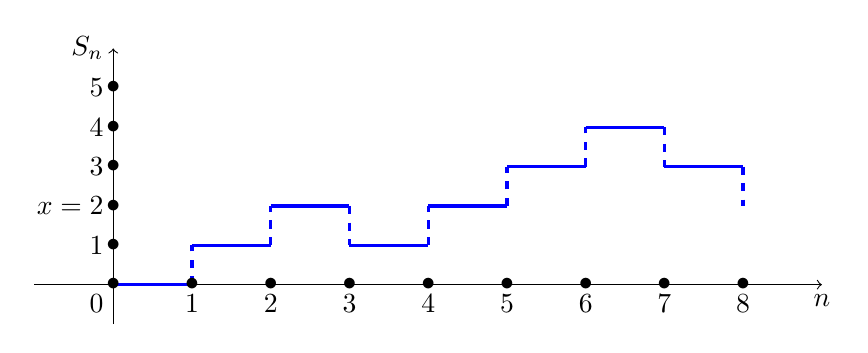
\begin{tikzpicture}
  %Origin and axis
  \coordinate (O) at (0,0);
  \draw[->] (-1,0) -- (9,0) coordinate[label = {below:$n$}] (xmax);
  \draw[->] (0,-0.5) -- (0,3) coordinate[label = {left:$S_n$}] (ymax);
  %Lower linear boundary

 
  %Stochastic process trajectory
  
  \draw (0,0) node[blue,left] {} node{};
  \draw[very thick,blue,-] (0,0) -- (1,0) node[pos=0.5, above] {} ;
  \draw[very thick,dashed,blue] (1,0) -- (1,0.5) node[pos=0.5, right] {};
  \draw[very thick,blue,-] (1,0.5) -- (2,0.5) node[pos=0.5, above] {};
  \draw[very thick,dashed,blue] (2,0.5) -- (2,1) node[pos=0.5, right] {};
  \draw[very thick,blue,-] (2,1) -- (3,1) node[pos=0.5, above] {};
  \draw[very thick,dashed,blue] (3,1) -- (3,0.5) node[pos=0.5, right] {};
  \draw[very thick,blue,-] (3,0.5) -- (4,0.5)node[pos=0.5, above] {};
  \draw[very thick,dashed,blue] (4,0.5) -- (4,1) node[pos=0.5, right] {};  
  \draw[very thick,blue,-] (4,1) -- (5,1) node[pos=0.5, above] {};
  \draw[very thick,dashed,blue] (5,1) -- (5,1.5) node[pos=0.5, right] {};  
  \draw[very thick,blue,-] (5,1.5) -- (6,1.5) node[pos=0.5, above] {};
  \draw[very thick,dashed,blue,-] (6,1.5) -- (6,2) node[pos=0.5, above] {};
   \draw[very thick,blue,-] (6,2) -- (7,2) node[pos=0.5, above] {};
    \draw[very thick,dashed,blue,-] (7,2) -- (7,1.5) node[pos=0.5, above] {};
     \draw[very thick,blue,-] (7,1.5) -- (8,1.5) node[pos=0.5, above] {};
     \draw[very thick,dashed,blue,-] (8,1.5) -- (8,1) node[pos=0.5, above] {};
  %Jump Times
  \draw (1,0) node[black,below] {$1$} node{ \color{black}$\bullet$};
  \draw (2,0) node[black,below] {$2$} node{ \color{black}$\bullet$};
  \draw (3,0) node[black,below] {$3$} node{ \color{black}$\bullet$};
  \draw (4,0) node[black,below] {$4$} node{ \color{black}$\bullet$};
  \draw (5,0) node[black,below] {$5$} node{ \color{black}$\bullet$};
  \draw (6,0) node[black,below] {$6$} node{ \color{black}$\bullet$};
  \draw (7,0) node[black,below] {$7$} node{ \color{black}$\bullet$};
  \draw (8,0) node[black,below] {$8$} node{ \color{black}$\bullet$};
  %Level of the counting process
   \draw (0,0) node[black,below left] {$0$} node{ \color{black}$\bullet$};
   \draw (0,0.5) node[black,left] {$1$} node{ \color{black}$\bullet$};
   \draw (0,1) node[black,left] {$x=2$} node{ \color{black}$\bullet$};
   \draw (0,1.5) node[black,left] {$3$} node{ \color{black}$\bullet$};
   \draw (0,2) node[black,left] {$4$} node{ \color{black}$\bullet$};
   \draw (0,2.5) node[black,left] {$5$} node{ \color{black}$\bullet$};

  % %Aggregated Capital gains
%  \draw (0,1.5) node[blue,below right] {$\mu_1$} node{ \color{blue}$-$};
%  \draw (0,2.25) node[blue,left] {$\mu_2$} node{ \color{blue}$-$};
%  \draw (0,3.75) node[blue,left] {$\mu_3$} node{ \color{blue}$-$};
  %Ruin time = First-crossing time time
%  \draw (5,0) node[black,above right] {${\tau_0}_u$} node{ \color{black}$\times$};
%  \draw[dotted,black] (0,3.28) -- (5,3.28);
%  \draw[dotted,black] (5,0) -- (5,3.28);
\end{tikzpicture}
\label{subfig:time_reversed_ds_RW_time}
}
\end{center}
\caption{Another look at the first hitting time problem.}
\label{fig:time_reversed_double_spending_time}
\end{figure}
We have equivalently
$$
\mathbb{P}_x(\tau_0=n) = \mathbb{P}(S_k>0,\text{ }1\leq k\leq n|S_n = x, S_0 = 0)\mathbb{P}_0(S_n = x|S_0=0),
$$
and 
$$
\mathbb{P}(S_k>0,\text{ }1\leq k\leq n|S_n = x, S_0 = 0) = \frac{x+(n-x)/2-(n-x)/2}{n} = \frac{x}{n}.
$$
For proof of the ballot theorem, see \citet{Renault2007}. For a general formulation and application to queueing see \citet{Takacs1962}.
\end{remark}
To complete the proof, we just note that 
$$
\mathbb{P}_x(X_n = 0) = \binom{n}{(n-x) / 2}p^{(n-x) / 2}q^{(n
+x) / 2}
$$
as it corresponds to a trajectory of $(X_n)_{n \geq0}$ starting at $X_0 = x$ ending at $0$ made of $(n-x)/2$ upward jumps and $(n+x)/2$ downward one.
\end{proof}
Just like in the previous section, the actual double spending time depends on the value of the random variable $Z = (\alpha -M)_+$.

\section{Counting process model}\label{sec:counting_process}
Our aim is to go from the discrete time framework of the previous section to a continuous time. To do so, we will model the length of the blockchain as counting processes. We will consider renewal processes and more specifically Poisson processes. We start by giving some reminders on the exponential distribution and counting processes before studying the double spending time distribution.

\subsection{Poisson process, Exponential distributions and friends}\label{sssec:exp_distribution}
\begin{definition}\label{def:counting_process}
A counting process $(N_t)_{t\geq0}$ is a continuous time stochastic process that counts the occurence of an event over time such that
\begin{equation*}
N_0=0\text{ and }N_t=\sum_{k=1}^{+\infty}\mathbb{I}_{T_k\leq t}.
\end{equation*}
where $T_1,T_2,T_3,\ldots$ denote the arrival times, with the convention that $T_0=0$. Let $\Delta^T_0,\Delta^T_1,\Delta^T_2,\ldots$ be the sequence of inter-arrival times defined as
$$
\Delta^T_k=T_{k+1}-T_{k}\text{, }k=0,1,2\ldots.
$$
\end{definition}
A trajectory of a counting process is given in 
\begin{figure}[!h]
\begin{center}
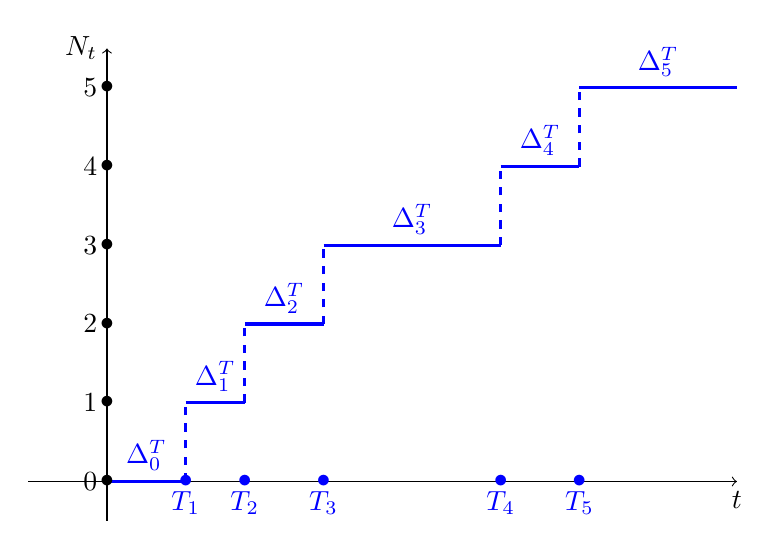
\begin{tikzpicture}[scale=1]
  %Origin and axis
  \coordinate (O) at (0,0);
  \draw[->] (-1,0) -- (8,0) coordinate[label = {below:$t$}] (xmax);
  \draw[->] (0,-0.5) -- (0,5.5) coordinate[label = {left:$N_t$}] (ymax);
  %Lower linear boundary


  %Stochastic process trajectory

  \draw (0,0) node[blue,left] {} node{};
  \draw[very thick,blue,-] (0,0) -- (1,0) node[pos=0.5, above] {$\Delta^T_0$} ;
  \draw[very thick,dashed,blue] (1,0) -- (1,1) node[pos=0.5, right] {};
  \draw[very thick,blue,-] (1,1) -- (1.75,1) node[pos=0.5, above] {$\Delta^T_1$};
  \draw[very thick,dashed,blue] (1.75,1) -- (1.75,2) node[pos=0.5, right] {};
  \draw[very thick,blue,-] (1.75,2) -- (2.75,2) node[pos=0.5, above] {$\Delta^T_2$};
  \draw[very thick,dashed,blue] (2.75,2) -- (2.75,3) node[pos=0.5, right] {};
  \draw[very thick,blue,-] (2.75,3) -- (5,3)node[pos=0.5, above] {$\Delta^T_3$};
  \draw[very thick,dashed,blue] (5,3) -- (5,4) node[pos=0.5, right] {};
  \draw[very thick,blue,-] (5,4) -- (6,4) node[pos=0.5, above] {$\Delta^T_4$};
  \draw[very thick,dashed,blue] (6,4) -- (6,5) node[pos=0.5, right] {};
  \draw[very thick,blue,-] (6,5) -- (8,5) node[pos=0.5, above] {$\Delta^T_5$};
  %Jump Times
  \draw (1,0) node[blue,below] {$T_1$} node{ \color{blue}$\bullet$};
  \draw (1.75,0) node[blue,below] {$T_2$} node{ \color{blue}$\bullet$};
  \draw (2.75,0) node[blue,below] {$T_3$} node{ \color{blue}$\bullet$};
  \draw (5,0) node[blue,below] {$T_4$} node{ \color{blue}$\bullet$};
  \draw (6,0) node[blue,below] {$T_5$} node{ \color{blue}$\bullet$};
  %Level of the counting process
   \draw (0,0) node[black,left] {$0$} node{ \color{black}$\bullet$};
   \draw (0,1) node[black,left] {$1$} node{ \color{black}$\bullet$};
   \draw (0,2) node[black,left] {$2$} node{ \color{black}$\bullet$};
   \draw (0,3) node[black,left] {$3$} node{ \color{black}$\bullet$};
   \draw (0,4) node[black,left] {$4$} node{ \color{black}$\bullet$};
   \draw (0,5) node[black,left] {$5$} node{ \color{black}$\bullet$};
\end{tikzpicture}
\end{center}
\caption{Trajectory of the counting process $(N_t)_{t\geq0}$.}
\label{fig:trajectory_counting_process}
\end{figure}
\begin{definition}\label{def_poisson_process}
A Poisson process $(N_t)_{t\geq0}$ is a counting process whose inter-arrival times are \iid exponential random variables.
\end{definition}
\begin{remark}\label{def_renewal_process}
A Poisson process belongs to the family renewal processes which are counting process with \iid inter-arrival times.
\end{remark}
\begin{definition}\label{def:exp_dist}
A random variable $X$ is exponentially distributed $X\sim\ExpDist(\lambda)$ if it has \pdf
$$
f_X(x) =\begin{cases} 
\lambda\e^{-\lambda x},&\text{ if }x>0,\\
0,&\text{ otherwise}.
\end{cases}
$$
\end{definition}
For some reasons, we need to introduce the joint distribution of the order statistics of a uniform random sample.
\begin{prop}\label{def:uniform_OS_dist}
Let $U_1,\ldots, U_n$ be a sample of \iid uniform random variables on $(a,b)$. Denote by 
$$
U_{1:n}\leq U_{2:n}\leq\ldots\leq U_{n:n}
$$
the order statistics of such a sample. The joint distribution of $(U_{(1)},\ldots,  U_{(n)})$ is given by 
$$
f_{(U_{1:n},\ldots, U_{n:n})}(u_1,\ldots, u_n)=\frac{n!}{(b-a)^n}\mathbb{I}_{a<u_1<\ldots< u_n<b}(u_1,\ldots, u_n).
$$
and we denote $(U_{1:n},\ldots,  U_{n:n})\sim \text{OS}_n([a,b])$
\end{prop}
\begin{proof}
Let $g:\mathbb{R}^n\mapsto \mathbb{R}_+$ be measurable and bounded. We have that
$$
\mathbb{E}[g(U_{1:n},\ldots,U_{n:n})]=\mathbb{E}\left[\sum_{\sigma\in\mathcal{S}_n}
g(U_{\sigma(1)},\ldots,U_{\sigma(n)})
\mathbb{I}_{U_{\sigma(1)} <\ldots< U_{\sigma(n)}}
\right]
$$
where $\mathcal{S}_n$ the set of all the permutation of $\{1,\ldots,n \}$. We note that
\begin{eqnarray*}
\mathbb{E}\left[g(U_{\sigma(1)},\ldots,U_{\sigma(n)})
\mathbb{I}_{U_{\sigma(1)} <\ldots< U_{\sigma(n)}}
\right]&=& \mathbb{E}\left[g(U_{1},\ldots,U_{n})
\mathbb{I}_{U_{1} <\ldots< U_{n}}\right]\\
&=&\int_{\mathbb{R}^{n}}g(u_{1},\ldots,u_{n})
\mathbb{I}_{u_{1} <\ldots< u_{n}}\frac{1}{(b-a)^n}\text{d}\lambda_{n}(u_1,\ldots, u_n).
\end{eqnarray*}
It then follows that
$$
\mathbb{E}[g(U_{1:n},\ldots,U_{n:n})]=\int_{\mathbb{R}^{n}}g(u_{1},\ldots,u_{n})
\mathbb{I}_{u_{1} <\ldots< u_{n}}\frac{n!}{(b-a)^n}\text{d}\lambda_{n}(u_1,\ldots, u_n).
$$
\end{proof}
We require some additional result about the gamma distribution.
\begin{prop}\label{prop:erlang_dist}
Let $\Delta^T_1,\ldots, \Delta^T_n$ be \iid exponential $\text{Exp}(\lambda)$ random variables, define the sequence $T_k=\sum_{i=1}^{k}\Delta^T_i, k=1,\ldots, n$.
\begin{enumerate}
\item The $T_{k}$'s are gamma distributed, $T_{k}\sim\GammaDist(k,\lambda)$ with \pdf 
$$
f_{T_k}(t)=\frac{t^{k-1}e^{-\lambda t}\lambda^k}{\Gamma(k)},\text{ }t>0,
$$
where $\Gamma(k) = \int_{0}^{\infty}\e^{- x}x^{k-1}\text{d}x$.
\item The joint distribution of $(T_1,\ldots, T_n)$ has \pmf given by
$$
f_{(T_1,\ldots, T_n)}(t_1,\ldots, t_n)=\lambda^n e^{-\lambda t_n }\mathbb{I}_{0<t_1<\ldots< t_n}(t_1,\ldots, t_n)
$$
\item $[(T_1,\ldots, T_n)|T_{n+1}=t]\sim \text{OS}_{n}([0,t])$
\end{enumerate}
\end{prop}
\begin{proof}
\begin{enumerate}
\item We use induction on $k\geq1$. For $k=1$ we have that $\Delta^T_1= T_1$ so the property holds. Assume that the property hold true for some $k$ and consider $k+1$. We note that $T_{k+1}=T_k+\Delta^T_{k+1}$ then
\begin{eqnarray*}
f_{T_{k+1}}(t)&=&\int_{0}^{t}f_{T_k}(x)f_{\Delta^T_{k+1}}(t-x)\text{d}x\\
&=&\int_{0}^{t}\frac{x^{k-1}e^{-\lambda x}\lambda^k}{(k-1)!}\lambda e^{-\lambda(t-x)}\text{d}x\\
&=&\frac{e^{-\lambda t}\lambda^{k+1}}{(k-1)!}\frac{t^k}{k}=\frac{t^k e^{-\lambda t}\lambda^{k+1}}{k!}.
\end{eqnarray*}
\begin{exercise}
Can you propose another way to show this result? Without using induction.
\end{exercise}
\item Let $g:\mathbb{R}^n\mapsto \mathbb{R}_+$ be measurable and bounded, we have
\begin{eqnarray*}
\mathbb{E}[g(T_{1},\ldots,T_n)]&=& \mathbb{E}[g(\Delta^T_{1},\Delta^T_1+\Delta^T_2\ldots,\Delta^T_1+\ldots+ \Delta^T_n)]\\
&=&\int_{\mathbb{R}^n}g(t_{1},\ldots,t_1+\ldots+ t_n)f_{(\Delta^T_{1},\ldots,\Delta^T_n)}(t_1,\ldots,t_n)\text{d}\lambda_n(t_{1},\ldots,t_n)\\
&=&\int_{\mathbb{R}_+^n}g(t_{1},\ldots,t_1+\ldots+ t_n)\lambda^n\e^{-\lambda(t_1+\ldots+t_n)}\text{d}\lambda_n(t_{1},\ldots,t_n)\\
\end{eqnarray*}
Let us apply the following change of variable 
$$
\Phi:(u_{1},\ldots,u_n)\mapsto(u_1, u_{2}-u_1,\ldots,u_n-u_{n-1}):=(t_1,\ldots, t_n),$$
minding the change in the integration domain as 
$$
\Phi(\mathbb{R}_+\times ]u_1,\infty[\times \ldots\times ]u_{n-1},\infty[) = \mathbb{R}^n_+ 
$$
and the Jacobian $\left|\frac{\text{d}\Phi}{\text{d}u}\right|=1$. It follows that
$$
\mathbb{E}[g(T_{1},\ldots,T_n)]=\int_{\mathbb{R}^n} g(u_1,\ldots, u_n)\lambda^{n}e^{-\lambda u_n}\mathbb{I}_{0<u_1<\ldots<u_n}(u_1,\ldots, u_n)\text{d}\lambda_{n}(u_1,\ldots, u_n).
$$
\item We have that 
\begin{eqnarray*}
f_{T_1,\ldots, T_n|T_{n+1}}(t_1,\ldots,t_n|t)
&=&\frac{f_{T_1,\ldots, T_n,T_{n+1}}(t_1,\ldots,t_n,t)}{f_{T_{n+1}(t)}}\\
&=&\frac{n!}{t^n}\mathbb{I}_{0<t_1<\ldots< t_n<t}(t_1,\ldots, t_n, t).
\end{eqnarray*}
\end{enumerate}
\end{proof}
The fact that the Poisson process is a Levy process will be useful later on, so here it is
\begin{prop}
Provided that $\{N_t=n\}$, the jump times $T_1,\ldots,T_n$ have the same distribution as the order statistic of an \iid sample of $n$ uniform random variable on $(0,t)$, namely it holds that
$$
[T_1,\ldots,T_n|N_t=n]\sim \left(U_{1:n}(0,t),\ldots, U_{n:n}(0,t)\right).
$$
\end{prop}
\begin{proof}
We have
\begin{eqnarray*}
&&\mathbb{E}\left[g(T_1,\ldots, T_n)|N_t = n\right]\\
&=&\frac{\mathbb{E}\left[g(T_1,\ldots, T_n)\mathbb{I}_{N_t = n}\right]}{\mathbb{P}(N_t = n)}\\
&=&\frac{\mathbb{E}\left[g(T_1,\ldots, T_n)\mathbb{I}_{T_n \leq t}\mathbb{I}_{T_{n+1} > t}\right]}{\mathbb{P}(N_t = n)}\\
&=&\frac{n!}{e^{-\lambda t}(\lambda t)^n}\int_{\mathbb{R}^{n+1}}g(t_1,\ldots, t_n)\mathbb{I}_{t_n\leq t<t_{n+1}}(t_n,t_{n+1})f_{T_1,\ldots, T_{n+1}}(t_1,\ldots, t_{n+1})\text{d}\lambda_{n+1}(t_1,\ldots, t_{n+1})\\
&=&\frac{n!}{e^{-\lambda t}(\lambda t)^n}\int_{\mathbb{R}^{n}}\int_{t}^{+\infty}g(t_1,\ldots, t_n)\mathbb{I}_{0<t_1<\ldots t_n\leq t}(t_1,\ldots,t_{n})\lambda^{n+1} e^{-\lambda t_{n+1}}\text{d}\lambda_{n+1}(t_1,\ldots, t_{n+1})\\
&=&\frac{n!}{e^{-\lambda t}(\lambda t)^n}\int_{\mathbb{R}^{n}}g(t_1,\ldots, t_n)\mathbb{I}_{0<t_1<\ldots t_n\leq t}(t_1,\ldots,t_{n})\lambda^{n} \text{d}\lambda_{n}(t_1,\ldots,t_n)\e^{-\lambda t}\\
&=&\int_{\mathbb{R}^{n}}g(t_1,\ldots, t_n)\frac{n!}{t^n}\mathbb{I}_{0<t_1<\ldots t_n\leq t}(t_1,\ldots,t_{n})\text{d}\lambda(t_1,\ldots,t_{n} ).
\end{eqnarray*}
\end{proof}
\noindent The order statistic property of the Poisson process will be useful to solve the first hitting time problem arising later on. 


\subsection{Levy process and continuous time martingale}\label{ssec:levy_mart}
Levy processes are the continuous time equivalent of random walks. Let $(\Omega,\F,\F_t,\Prob)$ be a filtered probability space and $X$ a $\F_t-$adapted stochastic process.
\begin{definition}
$X$ is a Levy process if
\begin{enumerate}
    \item $X_0 = 0$
    \item $X_t - X_s \overset{\mathcal{D}}{=}X_{t-s}\text{ (Stationary increments)}$
    \item For all $n\in\mathbb{N}$ and $0\leq s_1\leq t_1\leq s_2\leq t_2\leq \ldots\leq s_n\leq t_n<\infty$, the increments
    $$
    X_{t_i}-X_{s_i},\text{ }i = 1,\ldots, n,
    $$
    are independent.
    \item The trajectories of $X$ are càdlàg (right-continuous and left-limited)
\end{enumerate}
\end{definition}

\begin{prop}
The following statements are equivalent
\begin{enumerate}
\item $(N_t)_{t\geq 0}$ is a Poisson process
\item The stochastic process $(N_t)_{t\geq 0}$ has
\begin{itemize}
\item[(i)] independent increments, it means that for $0<t_1\leq\ldots\leq t_n$, the random variables
$N_{t_1},N_{t_2}-N_{t_1},\ldots,N_{t_{n}}-N_{t_{n-1}}$
are independent.
\item[(ii)] stationnary increments in the sense that the event frequency distribution over some time period of duration $s>0$ only depends on $s$. Indeed, we have that 
$$
N_{t+s}-N_t\sim\PoissonDist(\lambda s),\text{ for }s,t\geq 0.
$$
\end{itemize}
\end{enumerate}
Poisson processes are prominent examples of Levy processes.
\end{prop}
\begin{proof}
\underline{$1 \Rightarrow 2$}\\
Assume that $(N_t)_{t\geq0}$ is a Poisson process and let $0<t_1<\ldots <t_n$ be some times. Consider the folowing probability 
$$
\mathbb{P}\left(N_{t_1} = j_1, N_{t_2}-N_{t_1} = j_2,\ldots, N_{t_n}-N_{t_{n-1}} = j_n\right)
$$
such that $j_1,\ldots, j_n\in \mathbb{N}$. We can rewrite it as 
$$
\mathbb{P}\left(T_{k_1}\leq t_1<T_{k_1+1}, T_{k_2}\leq t_2<T_{k_2+1},\ldots, T_{k_n} \leq t_n<T_{k_n+1}\right),
$$
where $k_i = j_1 + \ldots +j_i, i = 1,\ldots, n$. Conditionning with respect to  $T_{k_n+1}$ yields
\begin{eqnarray*}
&&\mathbb{P}\left(T_{k_1}\leq t_1<T_{k_1+1}, T_{k_2}\leq t_2<T_{k_2+1},\ldots, T_{k_n}\leq t_n<T_{k_n+1}\right)\\
&=&\int_{t_n}^{+\infty}\mathbb{P}\left(T_{k_1}<t_1<T_{k_1+1}, T_{k_2}<t_2<T_{k_2+1},\ldots, T_{k_n}<t_n|T_{k_n +1}=t\right)f_{T_{k_n+1}}(t)\text{d}\lambda(t)\\
&=& \int_{t_n}^{+\infty}\binom{k_n}{j_1,\ldots, j_n}\left(\frac{t_1}{t}\right)^{j_1}\left(\frac{t_2-t_1}{t}\right)^{j_2}\ldots \left(\frac{t_n-t_{n-1}}{t}\right)^{j_n}\frac{e^{-\lambda t}t^{k_n}\lambda^{k_n + 1}}{k_n!}\text{d}\lambda(t)\\
&=&\frac{e^{-\lambda t_1}\left(t_1\right)^{j_1}}{j_1!}\frac{\left(t_2-t_1\right)^{j_2}e^{-\lambda(t_2 - t_1)}}{j_2!}\ldots \frac{\left(t_n-t_{n-1}\right)^{j_n}e^{-\lambda(t_n - t_{n-1})}}{j_n!}
\end{eqnarray*}
From the second to the third equality we simply ask that amomg $k_n$ uniform random variables $j_1$ fall inside $(0,t_1)$, $j_2$ fall inside $(t_1,t_2)$, etc...


\noindent \underline{$2 \Rightarrow 1$}\\
We aim at showing that $(T_1,\ldots, T_n)$ has \pdf given by
\begin{equation}\label{eq:joint_density_arrival_times}
f_{T_1,\ldots, T_n}(t_1,\ldots, t_n)=\lambda^n e^{-\lambda t_n}\mathbb{I}_{0< t_1<\ldots<t_n}.
\end{equation}
Let $t_1,\ldots, t_n$ and $h$ be nonnegative real numbers such that
$$
t_1<t_1+h<t_2<\ldots<t_n<t_n+h,
$$ 
We have
\begin{eqnarray*}
&&\mathbb{P}(t_1<T_1<t_1+h,\ldots,t_n<T_1<t_n+h)\\
&=&\mathbb{P}(N_{t_1}=0,N_{t_1+h}-N_{t_1}=1,\ldots,N_{t_n}-N_{t_{n-1}+h}=0,N_{t_n+h}-N_{t_n}\geq 1)\\
&=&e^{-\lambda t_1}e^{-\lambda h}\lambda h e^{-\lambda [t_2-(t_1+h)]}e^{-\lambda h}\lambda h\ldots e^{-\lambda [t_n-(t_{n-1}+h)]}[1-e^{-\lambda h}] \\
&=&e^{-\lambda t_n}\lambda^{n-1}h^{n-1}[1-e^{-\lambda h}]\\
\end{eqnarray*}
Divide by $h^{n}$ and let $h$ go to $0$ to get \eqref{eq:joint_density_arrival_times}. After applying a change of variable (reciprocal of that used in the proof of \cref{prop:erlang_dist}) to recover the joint distribution of $(\Delta^{T}_1, \ldots, \Delta^{T}_n)$, we see that the later is actually that of an \iid sample of size $n$ of exponential random variables.
\end{proof}
\begin{definition}
The Laplace exponent of $X$ is given by
$$
\kappa(\theta) = \log \E(\e^{\theta X_1}).
$$
\end{definition}
\begin{prop}
We have
$$
\log \E(\e^{\theta X_t}) = \kappa(\theta)t,\text{ for }t\geq 0
$$
\end{prop}
\begin{proof}
Let $t\geq 0$ and $n\in \mathbb{N}$, we have
$$
X_t=\sum_{k=0}^{n-1}\left(X_{(k+1)\frac{t}{n}} - X_{k\frac{t}{n}} \right).
$$
It follows that
\begin{eqnarray*}
\E\left(e^{\theta X_t}\right)&=&\E\left(e^{\theta \sum_{k=0}^{n-1}\left(X_{(k+1)\frac{t}{n}} - X_{k\frac{t}{n}} \right)}\right)\\
&=&\prod_{k=0}^{n-1}\E\left(e^{\theta \left(X_{(k+1)\frac{t}{n}} - X_{k\frac{t}{n}} \right)}\right)\\
&=&\prod_{k=0}^{n-1}\E\left(e^{\theta X_{t/n}}\right)\\
&=&\E\left(e^{\theta X_{t/n}}\right)^n\\
\end{eqnarray*}
If we denote by
$$
\kappa_t(\theta) = \log \E\left(e^{\theta X_t}\right)
$$
then it holds that 
$$
\kappa_t(\theta) = n\kappa_{t/n}(\theta),
$$
$\forall t\geq 0$ and $\forall n\in \mathbb{N}$. Furthermore, for $m\in\mathbb{N}$, we have
$$
\kappa_m(\theta) = m\kappa(\theta)\text{ and }\kappa_m(\theta) = n\kappa_{m/n}(\theta).
$$
Hence
$$
\kappa_t(\theta) = t\kappa(\theta)\text{ pour }t\in\Q
$$
Consider $(t_n)_{n\geq 0}\in \Q\text{ (rational numbers)}$ such that $t_n\downarrow t\in \RL$, taking the limit yields
$$
\kappa_{t}(\theta) = t\kappa(\theta)\text{ pour }t\in\mathbb{R},
$$
thanks to the cadlag nature of the trajectories of $X$
\end{proof}
\begin{definition}\label{def:martingale_contd}
$X$ is a $\F_t$-martingale if it holds that
\begin{itemize}
    \item $\E(|X_t|)<\infty$ for $t\geq 0$
    \item $\E(X_t|\F_s) = X_s$ for every $s\leq t$.
\end{itemize}
\end{definition}


\begin{theo}\label{theo:optional_stopping_theorem_continuous_martingale}
Let $X$ be a martingale and $\tau$ be a bounded stopping time, then $(X_{\tau\land t})_{t\geq 0}$ is a martingale and we have that
$$
\E(X_\tau) = \E(X_0).
$$
\end{theo}
\begin{prop}[Wald's exponential martingale]\label{prop:Wald_martingale_Levy}
Let $X$ be a Levy process then the process 
$$
M_t = \exp\left[\theta X_t - t\kappa(\theta)\right],\text{ }t\geq 0.
$$
is a $\F_t$-martingale.
\end{prop}
\begin{proof}
Let $s\leq t$, we have
\begin{eqnarray*}
\E(M_t|\F_s)&=&\e^{-t\kappa(\theta)}\E\left[\e^{\theta X_t}|\F_s\right]\\
&=&\e^{-t\kappa(\theta)}\E\left[\e^{\theta (X_t-X_s) +\theta X_s}|\F_s\right]\\
&=&\e^{-t\kappa(\theta)}\e^{\theta X_s}\E\left[\e^{\theta (X_t-X_s)}\right]\\
&=&\e^{-t\kappa(\theta)}\e^{\theta X_s}\e^{(t-s)\kappa(\theta)}\\
&=&M_s\\
\end{eqnarray*}
\end{proof}


\subsection{Double spending probability}\label{ssec:double_spending_counting_process_dsp}
The \textit{Proof-of-Work} protocol implies a steady block arrival, every $10$ minnutes for the bitcoin blockchain. Each trial (of the network) for mining a block is independent of the others and leads to a success with very small probability, the overall number of successes is binomially distributed, very well approximated by a
Poisson random variable. This justifies the Poisson process assumption made in the sequel to model the block arrival.\\

\noindent Denote by $(x+ N_t)_{t\geq 0}$ and $(M_t)_{t\geq 0}$ the number of blocks found by the honest miners and the attackers respectively. Double spending occurs at time 
$$
\tau_0 = \inf\{t\geq0\text{ ; }x+N_t = M_t\}.
$$
Assume that $(N_t)_{t\geq 0}$ and $(M_t)_{t\geq 0}$ are Poisson processes with intensity $\lambda$ and $\mu$ such that $\lambda>\mu$. Let $(T_i)_{i\geq0}$ and $(S_i)_{i\geq0}$ be the arrival times of $(N_t)_{t\geq 0}$ and $(M_t)_{t\geq 0}$
The first-hitting problem along with its notation is illustrated in \cref{fig:ds_poisson_process_illustrated}.
\begin{figure}[!ht]
\begin{center}
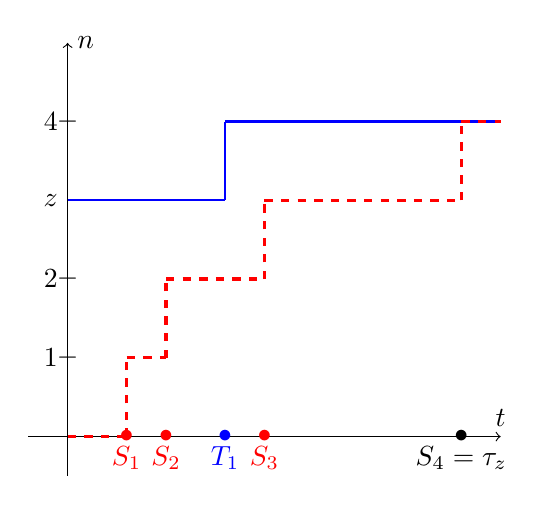
\begin{tikzpicture}
  %Origin and axis
  \coordinate (O) at (0,0);
  \draw[->] (-0.5,0) -- (5.5,0) coordinate[label = {above:$t$}] (xmax);
  \draw[->] (0,-0.5) -- (0,5) coordinate[label = {right:$n$}] (ymax);
 %Length of the honest chain
  \draw[thick,blue,-] (0,3) -- (2,3) node[pos=0.5, above] {} ;
  \draw[thick,blue] (2,3) -- (2,4) node[pos=0.5, above] {};
  \draw[thick,blue] (2,4) -- (5.5,4) node[pos=0.5, right] {};
  % %Length of the Malicious chain
  \draw[very thick,dashed,red,-] (0,0) -- (0.75,0) node[pos=0.5, above] {} ;
  \draw[very thick,dashed,red] (0.75,0) -- (0.75,1) node[pos=0.5, right] {};
  \draw[very thick,dashed,red] (0.75,1) -- (1.25,1) node[pos=0.5, above] {};
  \draw[very thick,dashed,red] (1.25,1) -- (1.25,2) node[pos=0.5, right] {};
  \draw[very thick,dashed,red] (1.25,2) -- (2.5,2) node[pos=0.5, above] {};
  \draw[very thick,dashed,red] (2.5,2) -- (2.5,3) node[pos=0.5, right] {};
  \draw[very thick,dashed,red] (2.5,3) -- (5,3) node[pos=0.5, right] {};
  \draw[very thick,dashed,red] (5,3) -- (5,4) node[pos=0.5, above] {};
  \draw[very thick,dashed,red] (5,4) -- (5.5,4) node[pos=0.5, above] {};
  %Jump Times of the malicious chain
  \draw (0.75,0) node[red,below] {$S_1$} node{ \color{red}$\bullet$};
  \draw (1.25,0) node[red,below] {$S_2$} node{ \color{red}$\bullet$};
  \draw (2.5,0) node[red,below] {$S_3$} node{ \color{red}$\bullet$};
  \draw (5,0) node[black,below] {$S_4=\tau_z$} node{ \color{black}$\bullet$};
  % %Jump Times of the honest chain
  \draw (2,0) node[blue,below] {$T_1$} node{ \color{blue}$\bullet$};
  % %Aggregated Capital gains
  \draw (0,1) node[black,left] {$1$} node{ \color{black}$-$};
  \draw (0,2) node[black,left] {$2$} node{ \color{black}$-$};
  \draw (0,3) node[black,left] {$z$} node{};
  \draw (0,4) node[black,left] {$4$} node{ \color{black}$-$};
  % %Ruin time = First-meeting time
  % \draw (7,0) node[black,below] {$\tau_z$} node{ \color{black}$\times$};
  % \draw[dotted,black] (7,3) -- (7,0);
\end{tikzpicture}
\end{center}
\caption{Illustration of the double spending problem within a continuous time framework.}
\label{fig:ds_poisson_process_illustrated}
\end{figure}
The double spending probability is given by the following result
\begin{theo}\label{theo:ds_probability_Poisson_process}
The double spending probability is given by 
$$
\mathbb{P}(\tau_0 < \infty) = \left(\frac{\mu}{\lambda}\right)^x.
$$
\end{theo}
\begin{proof}

Define the processes
$$
X_t = x + N_t - M_t
$$ 
and
$$
Y_t = x - X_t = M_t - N_t,\text{ }t\geq0.
$$
$(Y_t)_{t\geq0}$ is a L\'evy process such that $Y_t\rightarrow - \infty$ because $\lambda >\mu$. Recall that 
$$
\exp(\theta Y_t - t\kappa(\theta)), \text{ }t\geq 0,
$$
is a martingale. We would like to find $\gamma>0$ such that $\exp(\gamma Y_t)$. Consider the equation 
$$
\kappa(\theta) =\log\mathbb{E}\left(e^{\theta Y_1}\right) = 0.
$$
Tt is equivalent to 
$$
\mu \e^\theta + \lambda \e^{-\theta}- (\mu+\lambda) =0,
$$
which has two solutions: $0$ and 
$$
\gamma = \log\left(\frac{\lambda}{\mu}\right).
$$
It follows from \cref{prop:Wald_martingale_Levy} that $(\e^{\gamma Y_t})_{t\geq 0}$ is a martingale. We apply the optional stopping theorem (that's \cref{theo:optional_stopping_theorem_continuous_martingale}) to the process $\e^{\gamma Y_t}$ at $t\land\tau_0$. We have 
\[
\mathbb{E}(e^{\gamma Y_0}) = 1,
\]
and 
\[
\mathbb{E}(e^{\gamma Y_{\tau_0\land t}}) = \mathbb{E}(e^{\gamma Y_{\tau_0}}\mathbb{I}_{\tau_0 < t }) + \mathbb{E}(e^{\gamma Y_{t}}\mathbb{I}_{\tau_0 \geq  t }).
\]
We are going to take the limit $t\rightarrow \infty$. Note that 
\[
\tau_0  = \inf\{t\geq 0\text{ ; }x+N_t = M_t\} = \inf\{t\geq 0\text{ ; }X_t = 0\} = \inf\{t\geq 0\text{ ; }Y_t = x\}.
\]
We deduce that $Y_{\tau_0} = x$ and that $\e^{\gamma Y_{t}} < \e^{\gamma x}$ on $\{\tau_0 \geq t\}$. Applying the dominated convergence theorem yields
\[
\mathbb{E}(e^{\gamma Y_{\tau_0\land t}}) \underset{t\rightarrow \infty}{\rightarrow} e^{\gamma x}\Prob(\tau_0 < \infty).
\]
The identity 
\[
\mathbb{E}(e^{\gamma Y_0}) =\mathbb{E}(e^{\gamma Y_{\tau_0\land t}})
\]
holds for any $t$ including $t\rightarrow \infty$ which in turns leads to 
\[
1 = e^{\gamma x}\Prob(\tau_0 < \infty)\Leftrightarrow \mathbb{P}(\tau_0<\infty) = \left(\frac{\mu}{\lambda}\right)^x.
\]
\end{proof}
\subsection{Double spending time}\label{ssec:double_spending_counting_process_dst}
Just like in \cref{sssec:double_spending_rw_dst}, we are interested in the time required to complete a double spending attack. Accounting for the cost of electricity, we can approximate the operational cost per time unit by 
$$
c = \pi_W\cdot W\cdot q,
$$
where 
\begin{itemize}
  \item $\pi_W$ is the electricity cost
  \item $W$ is the electricity consumed by the network
  \item  $q$ is the attacker's hashpower
\end{itemize}
The double spending cost reduces to $\tau_z\cdot c$. the following result provides a formula for the \pdf of $\tau_z$.
\begin{theo}
If $(N_t)_{t\geq0}$ is a Poisson process and $(M_t)_{t\geq0}$ is a renewal process then the \textbf{p.d.f.} of $\tau_z$ is given by
\begin{equation}\label{eq:DS_time_pdf}
f_{\tau_0}(t)=\mathbb{E}\left[\frac{x}{x+N_t}f_{S_{N_t+x}}(t)\right],\text{ for }t\geq0,
\end{equation}
where $S_1, S_2, \ldots, $ denotes the arrival times of $(M_t)_{t\geq 0}$.
\end{theo}
\begin{proof}
The event $\{\tau_0\in(t,t+\text{d}t)\}$, for $t\geq0$, corresponds to the exact time at which the double-spending attack is successful as the malicious chain takes over the honest one. At time $t=0$, the honest chain is ahead by $x\geq 1$ blocks. Assuming that later, at time $t>0$, the honest miners manage to add $N_t=n\in\mathbb{N}$ blocks to the chain then the malicious chain must be of length $M(t^{-})=n+x-1$ at some time $t^{-}<t$ and jumps to the level $n+x$ exactly at $t$. Conditioning over the values of $\{N_t\text{ , }t\geq0\}$ yields
\begin{equation}\label{eq:Tauz}
\{\tau_0\in(t,t+\text{d}t)\}=\bigcup_{n=0}^{+\infty}\{\tau_0\in(t,t+\text{d}t)\}\cap\{N_t=n\}.
\end{equation}
In the case where $N_t=0$, the only requirement is that the $x^{\text{th}}$ jump of $(M_t)_{t\geq0}$ occurs at time $t$. It then follows that
\begin{equation}\label{eq:TauzNt0}
\{\tau_0\in(t,t+\text{d}t)\}\cap\{N_t=0\}=\{S_{x}\in(t,t+\text{d}t)\}\cap\{N_t=0\},
\end{equation}
and consequently
\begin{equation}\label{eq:PDFTauzNt0}
f_{\tau_0|N_t}(t|0)=f_{S_x}(t),\text{ }t\geq0,
\end{equation}
where $f_{\tau_0|N_t}(t|0)$ denotes the conditional \pdf of $\tau_0$ given that $N_t=0$. On the set $\{N_t\geq1\}$, one needs to make sure that $\{M_t\text{ , }t\geq0\}$ behaves properly by constraining its jump times so that it does not reach $N_s+x$ at any time $s<t$ and performs the $(n+x)^{\text{th}}$ jump at $t$. Hence, it holds that
\begin{equation*}
\{\tau_0\in(t,t+\text{d}t)\}\cap\{N_t\geq1\}=\bigcup_{n=1}^{+\infty}\bigcap_{k=1}^{n}\{T_k\leq S_{x+k-1}\}\cap\{S_{x+n}\in(t,t+\text{d}t)\}\cap\{N_t=n\}.
\end{equation*}
Applying the law of total probability yields
\begin{eqnarray}
&&\mathbb{P}\left(\{\tau_0\in(t,t+\text{d}t)\}\cap\{N(t)\geq1\}\right)\nonumber\\
&=&\sum_{n=1}^{+\infty}\mathbb{P}\left[\bigcap_{k=1}^{n}\{T_k\leq S_{x+k-1}\}\cap\{S_{x+n}\in(t,t+\text{d}t)\}\Big\rvert N(t)=n\right]\mathbb{P}[N(t)=n].\label{eq:LawOfTotalProbabilityTh1}
\end{eqnarray}
In virtue of the order statistic property, the successive jump times $(T_1,\ldots,T_n)$ are distributed as the order statistics $(U_{1:n}(0,t),\ldots,U_{n:n}(0,t))$ of a sample of $n$ \iid random variables uniformly distributed on $(0,t)$. The conditional probability in \eqref{eq:LawOfTotalProbabilityTh1} may be rewritten as
\begin{eqnarray}
&&\mathbb{P}\left[\bigcap_{k=1}^{n}\{U_{k:n}(0,t)\leq S_{x+k-1}\}\cap\{S_{x+n}\in(t,t+\text{d}t)\}\right]\nonumber\\
&=&\mathbb{P}\left[\bigcap_{k=1}^{n}\{U_{k:n}(0,1)\leq S_{x+k-1}/ t\}\cap\{S_{x+n}\in(t,t+\text{d}t)\}\right]\nonumber\\
&=&\mathbb{P}\left[\bigcap_{k=1}^{n}\{U_{k:n}(0,1)\leq S_{x+k-1}/t\}\big\rvert S_{x+n}\in(t,t+\text{d}t)\right]\mathbb{P}[S_{x+n}\in(t,t+\text{d}t)]\nonumber\\
&=&\mathbb{E}\left\{(-1)^{n}G_{n}[0\big\rvert S_{x}/t,\ldots, S_{x+n-1} / t] \big\rvert S_{x+n}\in(t,t+\text{d}t)\right\}\mathbb{P}[S_{x+n}\in(t,t+\text{d}t)],\nonumber\\
&=&(-1/t)^{n}\mathbb{E}\left\{G_{n}[0\big\rvert S_{x},\ldots, S_{x+n-1}] \big\rvert S_{x+n}\in(t,t+\text{d}t)\right\}\mathbb{P}[S_{x+n}\in(t,t+\text{d}t)],\nonumber\\
&&\label{eq:AGPolynomialsProof}
\end{eqnarray}
where $(G_n(.|.))_{n\geq 0}$ correspond to the sequence of A-G polynomials as defined in \cref{app:appell_AG_polynomials}. The last equation in \eqref{eq:AGPolynomialsProof} follows from using the first identity of \cref{prop:Appell_AG_polynomials_properties}.
Inserting \eqref{eq:AGPolynomialsProof} into \eqref{eq:LawOfTotalProbabilityTh1} and letting $\text{d}t$ be small enough yields
\begin{eqnarray}
f_{\tau_0|N(t)\geq1}(t)&=&\sum_{n=1}^{+\infty}(-1/t)^{n}\mathbb{E}\left\{G_{n}[0\big\rvert S_{x},\ldots,S_{x+n-1}] \big\rvert S_{x+n}=t\right\}\nonumber\\
&\times&f_{S_{x+n}}(t)\mathbb{P}[N(t)=n]\label{eq:cond_pdf_tau_N_greater_than_1}.
\end{eqnarray}
We further work on the AG polynomials to simplify the above expressions. We have that
\begin{eqnarray} 
\mathbb{E}\left\{G_{n}(0\big\rvert S_{x},\ldots,S_{x+n-1}) \rvert S_{x+n}=t\right\}&=& \mathbb{E}\left\{G_{n}(-S_x\rvert 0,\ldots,S_{x+n-1}-S_x) \rvert S_{x+n}=t\right\} \nonumber\\
&=& \mathbb{E}\left\{\mathbb{E}\left[G_{n}(-S_x\rvert 0,\ldots,S_{x+n-1}-S_x)\rvert S_{x+n}-S_x, S_{x+n}\right] \rvert S_{x+n}=t\right\} \nonumber\\
&=& \mathbb{E}\left\{(-S_x)(-S_x-S_{n+x}+S_x)^{n-1} \rvert S_{x+n}=t\right\} \nonumber\\
&=& (-1)^n\mathbb{E}\left\{S_x S_{n+x}^{n-1} \rvert S_{x+n}=t\right\} \nonumber\\
&=& (-1)^nt^{n-1}\frac{x}{x+n}t =(-t)^n\frac{x}{x+n} \label{eq:AG_polynomial_simplification}
\end{eqnarray}
Inserting \eqref{eq:AG_polynomial_simplification} into \eqref{eq:cond_pdf_tau_N_greater_than_1} yields
\begin{equation*}
f_{\tau_0|N_t\geq1}(t)=\sum_{n=1}^{+\infty}\frac{x}{x+n}f_{S_{x+n}}(t)\mathbb{P}(N_t=n)
\end{equation*}
The final step consists in adding the case $N_t=0$ to the sum, therefore writing
\begin{equation*}
f_{\tau_0}(t)=\sum_{n=0}^{+\infty}\frac{x}{x+n}f_{S_{x+n}}(t)\mathbb{P}(N_t=n)
\end{equation*}
which is equivalent to the announced result \eqref{eq:DS_time_pdf}.  
\end{proof}
\begin{exercise}
Assume that $(M_t)_{t\geq0}$ is a Poisson process with intensity $\mu$, compute 
\[
\mathbb{P}(\tau_0<\infty) = \int_0^{\infty}f_{\tau_0}(t)\text{d}t = \left(\frac{\mu}{\lambda}\right)^x.
\]
See \citet[Example 1]{Goffard2019} for the derivation. It is easier to verify the formula using python.  
\end{exercise}
\begin{remark}
Just like in the random walk framework of \cref{sec:double_spending_rw}, the number $z$ is actually a random variable defined as 
$$
Z = (\alpha - M_{T_\alpha})_+,
$$
where $T_\alpha$ is the arrival time of the $\alpha^{th}$ block in the main branch of the blockchain. If $(M_t)_{t\geq0}$ is a Poisson process with intensity $\mu$ then $M_{T_\alpha})$ is mixed Poisson distributed with parameter $\mu\cdot T_{\alpha}$. We have that 
\begin{eqnarray*}
\mathbb{P}(M_{T_\alpha} = m) &=& \int_{0}^{\infty}\frac{\e^{-\mu t}(\mu t)^m}{m!}\frac{\e^{-\lambda t}t^{\alpha-1}\lambda ^\alpha}{(\alpha -1)}\text{d}t\\
&=&\frac{\mu^m\lambda^{\alpha}}{m!(\alpha-1)!}\int_{0}^{\infty}\e^{-t(\mu + \lambda)}t^{m+\alpha-1}\text{d}t\\
&=&\binom{m+\alpha-1}{m}\left(\frac{\lambda}{\lambda+\mu}\right)^{\alpha}\left(\frac{\mu}{\lambda+\mu}\right)^{m}.
\end{eqnarray*}
The number of blocks found by the attacker until the vendor's transaction gets $\alpha$ confirmations is governed by a negative binomial distribution.
\end{remark}
\noindent For further results on the distribution of $\tau_0$ with different set of assumptions, the reader is referred to \citet{Goffard2019}.

\section{Appendix: Appell and Abel-Gontcharov polynomials}\label{app:appell_AG_polynomials}
\noindent Let $U=\{u_i, \, i\geq 1\}$ be a non-decreasing sequence of real numbers. To $U$ is attached a (unique) family of Appell polynomials of degree $n$ in $x$, $\{A_{n}(x\vert U),\, n\geq 0\}$ defined as follows.
\begin{definition} 
Starting with $A_0(x\vert U)=1$, the $A_n(x\vert U)$'s satisfy the differential equations
\begin{equation}\label{eq:DifferentialEquationAppellPolynomial}
A_{n}^{(1)}(x|U)=nA_{n-1}(x|U),  
\end{equation}
with the border conditions
\begin{equation}\label{eq:Border AppellPolynomial}
A_{n}(u_{n}|U)=0, \quad n\geq 1.
\end{equation}
So, each $A_n$ has the integral representation
\begin{equation}\label{eq:IntegralRepresentationAppellPolynomials}
A_{n}(x|U)=n!\int_{u_{n}}^{x}\left[\int_{u_{n-1}}^{y_{n}}\text{d}y_{n-1} \ldots \int_{u_{1}}^{y_{1}}\text{d}y_{1}\right]\text{d}y_{n}, \quad n\geq 1.
\end{equation}
\end{definition}

In parallel, to $U$ is attached a (unique) family of Abel-Gontcharov (A-G) polynomials of degree $n$ in $x$, $\{G_{n}(x\vert U),\, n\geq 0\}$.
\begin{definition} 
Starting with $G_0(x\vert U)=1$, the $G_n(x\vert U)$'s satisfy the differential equations
\begin{equation}\label{eq:DifferentialEquationAGPolynomials}
G_n^{(1)}(x|U)=nG_{n-1}(x|{\cal E}U), 
\end{equation}
where ${\cal E}U$ is the shifted family $\{u_{i+1}, \, i\geq 1\}$, and with the border conditions
\begin{equation}\label{eq:Border AGPolynomial}
G_{n}(u_{1}|U)=0, \quad  n\geq 1.
\end{equation}
So, each $G_n$ has the integral representation
\begin{equation}\label{eq:IntegralRepresentationAGPolynomials}
G_{n}(x|U)=n!\int_{u_{1}}^{x}\left[\int_{u_{2}}^{y_{1}}\text{d}y_{2} \ldots \int_{u_{n}}^{y_{n-1}}\text{d}y_{n}\right]\text{d}y_{1}, \quad n\geq 1.
\end{equation}
\end{definition}
\noindent The Appell and A-G polynomials are closely related through the identity
\begin{equation}\label{eq:link_AG_Appell}
G_{n}(x|u_{1},\ldots,u_{n})=A_{n}(x|u_{n},\ldots,u_{1}), \quad n\geq 1.
\end{equation}
The two families (i.e. for all $n\geq 0$), however, are distinct and enjoy different properties. From \eqref{eq:IntegralRepresentationAppellPolynomials} and \eqref{eq:IntegralRepresentationAGPolynomials}, it is clear that the polynomials $A_n$ and $G_n$ can be interpreted in terms of the joint distribution of the vector $(U_{1:n},\ldots,U_{n:n})$. 
\begin{prop}
For $0\leq u_1 \leq \ldots \leq u_{n} \leq x \leq 1$,
\begin{equation}\label{eq:ProbabilisticInterpretationAppellPolynomials}
P[U_{(1)} > u_1, \ldots, U_{(n)} > u_{n}\, \mbox{ and }\, U_{(n)}\leq x]= 
A_n(x \vert u_1, \ldots, u_{n}), \quad n\geq1.
\end{equation}
For $0\leq x \leq u_1 \leq \ldots \leq u_{n} \leq 1$,
\begin{equation}\label{eq:ProbabilisticInterpretationAGPolynomials}
P[U_{(1)} \leq u_1, \ldots, U_{(n)} \leq u_{n}\, \mbox{ and }\, U_{(1)}> x]
= (-1)^n \, G_n(x \vert u_1, \ldots, u_{n}), \quad n\geq 1.
\end{equation}
\end{prop}
The representations \eqref{eq:ProbabilisticInterpretationAppellPolynomials} and \eqref{eq:ProbabilisticInterpretationAGPolynomials} will play a key role for solving first-hitting problem that involve Poisson processes. Numerically, it will be necessary to evaluate some special values of the polynomials. To this end, it is convenient to use the following recusive relations. 
\begin{prop} 
The Appell polynomials are computed through the expansion
\begin{equation}\label{eq:appell_polynomials_recursion_1}
A_{n}(x|U)=\sum_{k=0}^{n}\binom{n}{k}A_{n-k}(0|U)x^{k}, \quad n\geq 1,
\end{equation}
where the $A_{n}(0|U)$'s are obtained recursively from 
\begin{equation}\label{eq:appell_polynomials_recursion_2}
A_{n}(0|U)=-\sum_{k=1}^{n} \binom{n}{k} A_{n-k}(0|U)u_{n}^{k}, \quad n\geq1.
\end{equation}
The A-G polynomials are computed through the recursion
\begin{equation}\label{eq:recursion_AG_polynomials}
G_{n}(x|U)=x^{n}-\sum_{k=0}^{n-1} \binom{n}{k} u_{k+1}^{n-k} G_{k}(x|U), \quad n\geq 1.
\end{equation}
\end{prop}
\begin{proof}
The Maclaurin expansion of $A_n(x|U)$ gives \eqref{eq:appell_polynomials_recursion_1} as
$$
A_n(x|U) = \sum_{k = 0}^n\frac{A_n^{(k)}(0|U)}{k!}x^k = \sum_{k = 0}^n\binom{n}{k}A_{n-k}(0|U)x^k.
$$
Evaluation at $x = u_n$ then provides \eqref{eq:appell_polynomials_recursion_2}. Regarding \eqref{eq:recursion_AG_polynomials}, first note that 
$$
G_n^{(k)}(u_{k+1}|U) = \begin{cases}
1,&\text{ if }k = n,\\
0,&\text{ otherwise.}
\end{cases}
$$
Any polynomials $R(x)$ of degree $n$ can therefore be written as 
$$
R(x)=\sum_{k = 0}^n\frac{R^{(k)}(u_{k+1})}{k!}G_k(x|U).
$$
By expanding $x^n$ one gets \eqref{eq:recursion_AG_polynomials}.
\end{proof}
Hereafter are a couple of useful properties
\begin{prop}\label{prop:Appell_AG_polynomials_properties}
\begin{enumerate}
\item For any $a,b\in \mathbb{R}$, it holds that
\begin{equation}
A_{n}(x|a+bU) = b^n A_n\left((x-a)/b \, |U\right), \quad n\geq 1, \label{eq:LinearTransform}
\end{equation}
with the same identity for $G_n$.
\item We have 
\begin{eqnarray}
&&A_{n}(x|1,\ldots,n) = x^{n-1}(x-n), \label{eq:ExplicitExpressionIntAppellPolynomials}\\
&&G_{n}(x|0,\ldots,n-1)= x(x-n)^{n-1}.    \label{eq:ExplicitExpressionIntAGPolynomials}
\end{eqnarray}
\item Let $\{X_{n}\text{ , }n\geq1\}$ be a sequence of \iid nonnegative random variables, of partial sums $S_{n}=\sum_{k=1}^{n}X_{k}$ with $S_0=0$. Then, for $n\geq 1$,
\begin{eqnarray}
&&\mathbb{E} \left[A_{n}(x|S_{1},\ldots,S_{n})\vert S_{n}\right] = x^{n-1}(x-S_{n}), \label{eq:ExplicitExpressionPartialSumsAppellPolynomials}\\
&&\mathbb{E}\left[G_{n}(x|S_{0},\ldots,S_{n-1})\vert S_{n}\right] = x(x-S_{n})^{n-1}.    \label{eq:ExplicitExpressionPartialSumsAGPolynomials}
\end{eqnarray}
\end{enumerate} 
\end{prop}
\begin{proof}
\begin{enumerate}
  \item Let us use induction on $n\geq1$. Take $n = 1$, we have
  $$
  A_1(x|a + bu_1) = \int_{a+bu_1}^{x} A_1'(y|a+bu_1)\text{d}y = x - a - bu_1 
  $$
  and 
   $$
  A_1(x|u_1) = x-u_1.
  $$
  The property holds for $n = 1$. Assume that it holds true for some $n$ and consider $n+1$. We have
  \begin{eqnarray*}
  A_{n+1}(x|a+bU) &=& \int^{x}_{a+b u_{n+1}}A_{n+1}'(y|a+bU)\text{d}y\\
  &=& \int^{x}_{a+b u_{n+1}}nA_{n}(y|a+bU)\text{d}y\\
  &=&b^n\int^{x}_{a+b u_{n+1}}nA_{n}\left(\frac{y-a}{b}\Big|U\right)\text{d}y\\
  &=&b^{n+1}n\int^{\frac{x-a}{b}}_{u_{n+1}}A_{n}\left(z\Big|U\right)\text{d}y\\
  &=&b^{n+1}\int^{\frac{x-a}{b}}_{u_{n+1}}A_{n+1}'\left(z\Big|U\right)\text{d}y\\
  &=&b^{n+1}A_{n+1}\left(\frac{x-a}{b}\Big|U\right),
  \end{eqnarray*}
  so the property holds for $n+1$. No need to do the job for the $G_n(.|U)$'s thanks to \eqref{eq:link_AG_Appell}.
\item Again induction on $n\geq1$. Take $n = 1$, we have
$$
A_1(x|1) = x-1
$$
Assume that the result holds true for some $n$ and consider $n+1$. We have 
\begin{eqnarray*}
A_{n+1}(x|1,\ldots, n,n+1) &=& \int_{n+1}^{x}A_{n+1}'(y|1,2,\ldots, n+1)\text{d}y\\
&=& (n+1)\int_{n+1}^{x}A_{n}(y|1,2,\ldots, n)\text{d}y\\
&=& (n+1)\int_{n+1}^{x}y^{n-1}(y-n)\text{d}y\\
&=& x^n[x - (n + 1)]
\end{eqnarray*}
For identity \eqref{eq:ExplicitExpressionIntAGPolynomials}, write 
\begin{eqnarray*}
G_{n}(x|0,\ldots, n-1)&=&G_{n}(x-n|-n ,\ldots,-1)\\
&=&(-1)^nG_{n}(n-x|n,\ldots, 1)\\
&=&(-1)^nA_{n}(n-x|1,\ldots, n)\\
&=&(-1)^n(n-x)^{n-1}(-x)\\
&=&x(x-n)^{n-1}.
\end{eqnarray*}
\item Again induction on $n\geq1$. Take $n = 1$, we have
$$
\mathbb{E}[A_1(x|S_1)|S_1] = x-S_1
$$
Assume that the result holds true for some $n$ and consider $n+1$. We have 
\begin{eqnarray*}
\mathbb{E}\left[A_{n+1}(x|S_1,\ldots, S_n,S_{n+1})|S_{n+1}\right]&=&\mathbb{E}\left[\int_{S_{n+1}}^x A_{n+1}'(y|S_1,\ldots, S_n,S_{n+1})\text{d}y|S_{n+1}\right]\\
&=&(n+1)\mathbb{E}\left[\int_{S_{n+1}}^x A_{n}(y|S_1,\ldots, S_n)\text{d}y|S_{n+1}\right]\\
&=&(n+1)\int_{S_{n+1}}^x\mathbb{E}\left[A_{n}(y|S_1,\ldots, S_n)|S_{n+1}\right]\text{d}y\text{ (Fubini)}\\
&=&(n+1)\int_{S_{n+1}}^x\mathbb{E}\left\{\mathbb{E}\left[A_{n}(y|S_1,\ldots, S_n)|S_n,S_{n+1}\right]|S_{n+1}\right\}\text{d}y\\
&=&(n+1)\int_{S_{n+1}}^x\mathbb{E}\left\{\mathbb{E}\left[A_{n}(y|S_1,\ldots, S_n)|S_n\right]|S_{n+1}\right\}\text{d}y\\
&=&(n+1)\int_{S_{n+1}}^x\mathbb{E}\left[y^{n-1}(y-S_n)|S_{n+1}\right]\text{d}y\\
&=&(n+1)\int_{S_{n+1}}^xy^n-\frac{n}{n+1}S_{n+1}y^{n-1} \text{d}y\\
&=&x^n(x-S_{n+1})\\
\end{eqnarray*}
For identity \eqref{eq:ExplicitExpressionPartialSumsAGPolynomials}, write 
\begin{eqnarray*}
\mathbb{E}\left[G_{n}(x|S_0,\ldots, S_{n-1})|S_{n}\right]&=&\mathbb{E}\left[G_{n}(x-S_n|S_0 - S_n,\ldots, S_{n-1}-S_n)|S_{n}\right]\\
&=&(-1)^n\mathbb{E}\left[G_{n}(S_n-x|S_n,\ldots, S_{n}-S_{n-1})|S_{n}\right]\\
&=&(-1)^n\mathbb{E}\left[A_{n}(S_n-x|S_{n}-S_{n-1},\ldots, S_n)|S_{n}\right]\\
&=&(-1)^n(S_n-x -S_n)(S_n-x)^{n-1}\\
&=&x(x-S_n)^{n-1}.\\
\end{eqnarray*}
\end{enumerate}
\end{proof}
% \section{A tiny bit of insurance risk theory}\label{sec:insurance_risk_theory}
% In what follows we will use classical result from insurance risk theory and so we have to provide some context. The financial reserve of a nonlife insurance company can be modelled by a continuous time stochastic process $(R_t)_{t\geq0}$ defined as 
% \begin{equation}\label{eq:risk_process}
% R_t = u + P_t - L_t,\text{ }t\geq0
% \end{equation}
% where 
% \begin{itemize}
%   \item $X_0 = u>0$ are the initial reserves,
%   \item $(P_t)_{t\geq0}$ is the premium income process,
%   \item $(L_t)_{t\geq0}$ is the liability of the insurance company, that is the sum of all the compensations paid to to the policyholders.
% \end{itemize}
% The classical assumes that the premium are collected linearly in times at some rate $c$ per time unit. Namely, we have 
% $$
% P_t = c\cdot t.
% $$
% The number of claims is governed by a counting process $(N_t)_{t\geq0}$, usually a standard Poisson process with intensity $\lambda$. To each claim is associated a randomly sized compensation distributed as $U$. The claim sizes $U_1,U_2,\ldots$ form a sequence of \iid random variables independent from $N_t$. We therefore have 
% $$
% L_t = \sum_{k = 1}^{N_t}U_k.
% $$
% The name of the game is to compute the ruin probabilities 
% \begin{equation}\label{eq:ruin_probabilities}
% \psi(u,T) = \mathbb{P}(\tau_u \leq T),\text{ and }\psi(u) = \mathbb{P}(\tau_u < \infty),
% \end{equation} 
% where $\tau_u = \inf\{t\geq0\text{ ; }R_t \leq 0\}$ is the ruin time. This first hitting time problem is illustrated on \cref{fig:ruin_time_CL}
% \begin{figure} 
% \begin{center}
% \begin{tikzpicture}
%   %Origin and axis
%   \coordinate (O) at (0,0);
%   \draw[->] (-0.5,0) -- (5.5,0) coordinate[label = {below:$t$}] (xmax);
%   \draw[->] (0,-0.5) -- (0,4) coordinate[label = {right:$R_t$}] (ymax);
%    %Initial reserves
%   \draw (0,2) node[black,left] {$z$} node{};
%  % % %Length of the honest chain
%   \draw[thick, blue,-] (0,2) -- (2,3) node[pos=0.5, above] {};
%   \draw[thick, dashed, blue] (2,3) -- (2,1) node[pos=0.5, left] {\color{black}$U_1$};
%   \draw[thick, blue] (2,1) -- (3,1.5) node[pos=0.5, above] {};
%   \draw[thick, dashed, blue] (3,1.5) -- (3, 0.5) node[pos=0.5, left] {\color{black}$U_2$};
%   \draw[thick, blue] (3,0.5) -- (5, 1.5) node[pos=0.5, above] {};
%    \draw[thick, dashed, blue] (5,1.5) -- (5, -0.5) node[pos=0.5,above left] {\color{black}$U_3$};

%   %Block finding Times 
%   \draw (2,0) node[black,below] {$T_1$} node{ \color{black}$\bullet$};
%   \draw (3,0) node[black,below] {$T_2$} node{ \color{black}$\bullet$};
%   \draw (5,0) node[black,below left] {$\tau_u$} node{ \color{black}$\bullet$};
% \end{tikzpicture}
% \end{center}
% \label{fig:ruin_time_CL}
% \caption{Illustration of the classical insurance ruin problem}
% \end{figure}
% This enables to select an initial reserves level $u$ so that the ruin probability is low enough. The premium rate is usually set to compensate the losses due to claims with 
% $$
% \mathbb{E}(P_t) = (1+\eta)\mathbb{E}(L_t)\text{ or  equivalently } c = (1+\eta)\lambda\mathbb{E}(U).
% $$
% Define the claim surplus process as
% $$
% S_t = u - R_t = L_t-P_t,\text{ }t\geq 0.
% $$
% The following result is the counterpart of \cref{lem:wald_martingale_RW} for Lévy processes.
% \begin{prop}\label{prop:wald_martingale_levy}
% If $(S_t)_{t\geq0}$ is a L\'evy process then
% $$
% M_t = \exp\left[\theta S_t-t\kappa(\theta)\right]\text{, }t\geq0,\text{ and }\theta\in \mathbb{R}, 
% $$
% where $\kappa(\theta)=\log\mathbb{E}\left(e^{\theta S_1}\right)<\infty$, is a martingale.
% \begin{proof}
% Note that for a Levy process, we have that 
% \[
% \mathbb{E}(e^{\theta S_t}) =\mathbb{E}(e^\theta S_1)^t. 
% \]
% It follows that 
% \begin{eqnarray*}
% \mathbb{E}(M_t|\mathcal{F}_s) &=&\mathbb{E}\left\{\exp\left[\theta S_t-t\kappa(\theta)\right]|\mathcal{F}_s\right\} \\
% &=&\e^{-t\kappa(\theta)}\mathbb{E}\left\{\exp\left[\theta (S_t-S_s) + \theta S_s\right]|\mathcal{F}_s\right\}\\
% &=&\e^{-t\kappa(\theta)}\e^{\theta S_s}\mathbb{E}\left(\e^{\theta (S_t-S_s)}\right)\\
% &=&\e^{-t\kappa(\theta)}\e^{\theta S_s}\e^{(t-s)\kappa(\theta)}\\
% &=&\e^{\theta S_s -s\kappa(\theta)}.
% \end{eqnarray*}
% \end{proof}
% \end{prop}
% The infinite time horizon ruin probability may be evaluated using the following result.
% \begin{prop}\label{prop:ruin_proba_levy}
% If $S_t\overset{\textbf{a.s.}}{\rightarrow} -\infty$, and there exists $\gamma>0$ such that $\left(e^{\gamma S_t}\right)_{t\geq0}$ is a martingale then
% $$
% \mathbb{P}(\tau_u<\infty)=\frac{e^{-\gamma u}}{\mathbb{E}\left[e^{\gamma \xi(u)}|\tau_u<\infty\right]},
% $$
% where $\xi(u)=S_{\tau_u}-u$ denotes the deficit at ruin.
% \end{prop}
% \begin{proof}
% We apply the optionnal stopping theorem on $(e^{\gamma S_t})_{t\geq0}$ at time $T\land \tau_u$ for some $T>0$ to get 
% \begin{eqnarray*}
% 1 = \mathbb{E}\left(\e^{\gamma S_0}\right)&=& \mathbb{E}\left(\e^{\gamma S_{T\land \tau_u}}\right)\\  
% &=& \mathbb{E}\left(\e^{\gamma S_{\tau_u}}\mathbb{I}_{\tau_u<T} + \e^{\gamma S_{T}}\mathbb{I}_{\tau_u\geq T}\right).\\
% \end{eqnarray*} 
% Letting $T\rightarrow\infty$  yields
% \begin{eqnarray*}
% 1 &=&\mathbb{E}\left(\e^{\gamma S_{\tau_u}}\mathbb{I}_{\tau_u<\infty}\right)\\
% &=&\e^{\gamma u}\mathbb{E}\left(\e^{\gamma \xi(u))}|\tau_u<\infty\right)\psi(u),
% \end{eqnarray*} 
% thanks to $S_t\rightarrow -\infty$, monotone and dominated convergence ($\e^{\gamma S_{T}}<\e^{\gamma u}$ on $\{\tau_u\geq T\}$)
% \end{proof}
% We will use \cref{prop:ruin_proba_levy} to derive the double spending probability within a continuous time framework in the next sections.

% \section{Blockwitholding in PoW}\label{sec:blockwithholding}
% The constant operational cost and the infrequent capital gains make mining blocks on a \PoW blockchain a risky activity. One way to tackle this problem is to engage in blockwitholding strategy. The goal is to build up a stock of blocks and release them publicly at well chosen times so as to fork the chain and make a part of the mining activities of competitors worthless, depending on which branch is followed up in the longer run. We focus here on a simplified version\footnote{For the sake of tractability.} of the original blockwitholding strategy called selfish mining and described in \citet{Eyal2014}. \\

% \noindent We start by introducing a risk model to follow the financial reserves of a miner over time. The ruin probability and expected profit given that ruin did not occur plays teh role of risk and performace indicators which will allow us to compare the solo mining strategy to the selfish mining strategy.

% \subsection{Ruin and expected profit of a miner}\label{ssec:selfish_mining}
% A miner, referred to as Sam, starts operating with an initial surplus level $u>0$. Mining blocks generates steady operational costs of amount $c>0$ per unit of time, most notably due to electricity consumption. The entire network of miners appends blocks to the blockchain at an exponential rate $\lambda$, which means that the length of the blockchain over time is governed by a Poisson process $(N_t)_{t\geq0}$ with intensity $\lambda$. We assume that Sam owns a fraction $q\in(0,1/2)$ of the overall computing power, which implies that each block is published by Sam with a probability $q$. The number of blocks found by Sam and therefore the number of rewards of size $b>0$ he collects up to time $t\geq 0$ is a thinned Poisson process $(\tilde{N}_t)_{t\geq0}$ with intensity $\lambda$ and thinning parameter $q$. Sam's surplus $R_t$ at time $t$ is then given by  
% \begin{equation}\label{eq:surplus_protocol}
% R_t = u + b\cdot\tilde{N}_t - c\cdot t,\qquad t\ge 0.
% \end{equation}
% The stochastic process $(R_t)_{t\geq0}$ is referred to as the dual risk process in risk theory, see for instance \citet{Avanzi2007}. Our goal is to measure the profitability of mining blocks on the blockchain, but subject to a ruin constraint. In this context, the time of ruin $\tau_u = \inf\{t\geq0:\text{ }R_t = 0\}$ is defined as the first time when the surplus reaches zero, i.e.\ the miner runs out of money and cannot continue to operate. 
% \begin{figure}[!ht]
% \begin{center}
% \begin{tikzpicture}
%   %Origin and axis
%   \coordinate (O) at (0,0);
%   \draw[->] (-0.5,0) -- (5.5,0) coordinate[label = {below:$t$}] (xmax);
%   \draw[->] (0,-0.5) -- (0,4) coordinate[label = {right:$R_t$}] (ymax);
%    %Initial reserves
%   \draw (0,3) node[black,left] {$u$} node{};
%  % % %Length of the honest chain
%   \draw[thick, blue,-] (0,3) -- (2,1) node[pos=0.5, above] {};
%   \draw[thick, dashed, blue] (2,1) -- (2,2) node[pos=0.5, above left] {\color{black}$b$};
%   \draw[thick, blue] (2,2) -- (3.5,0.5) node[pos=0.5, above] {};
%   \draw[thick, dashed, blue] (3.5,0.5) -- (3.5, 1.5) node[pos=0.5, above left] {\color{black}$b$};
%   \draw[thick, blue] (3.5,1.5) -- (5, 0) node[pos=0.5, above] {};

%   %Block finding Times 
%   \draw (2,0) node[black,below] {$T_1$} node{ \color{black}$\bullet$};
%   \draw (3.5,0) node[black,below] {$T_2$} node{ \color{black}$\bullet$};
%   \draw (5,0) node[black,below] {$\tau_u$} node{ \color{black}$\bullet$};
% \end{tikzpicture}
% \end{center}
% \caption{Ruin time in the miner risk model}
% \label{fig:ruin_time_miner}
% \end{figure}
% The riskiness of the mining business may be assessed via the finite-time and infinite-time horizon ruin probabilities defined as 
% \begin{equation}\label{eq:ruin_probabilities}
% \psi(u,t) = \mathbb{P}(\tau_u\leq t),\text{ and }\psi(u)=\mathbb{P}(\tau_u<\infty), 
% \end{equation}
% respectively. The rewards earned through mining must in expectation exceed the operational cost per time unit. The latter condition translates into $q\lambda b > c$, and is referred to as the net profit condition in standard risk theory, see \citet{Asmussen_2010}. In particular, this implies $\psi(u)<1$, i.e.\ ruin does not occur almost surely. The profitability for a time horizon $t>0$ is now measured by
% \begin{equation}\label{eq:value_function_finite_time}
% V(u,t) = \mathbb{E}(R_t\cdot \mathbb{I}_{\tau_u>t}),
% \end{equation}
% Correspondingly, $V(u,t)$ is the expected surplus level at time $t$, where in the case of ruin up to $t$ this surplus is $0$ (i.e., due to the ruin event the surplus is frozen in at $0$). In terms of a conditional expectation, one can equivalently express $V(u,t)$ as the probability to still be alive at $t$ times the expected value of the surplus at that time given that ruin has not occurred:
% \[V(u,t)= (1-\psi(u,t))\cdot \mathbb{E}(R_t\vert {\tau_u>t}).\]
%  The following result provides formulas for the ruin probabilities and $V(u,t)$ in this setting.
% \begin{prop}\label{prop:ruin_proba_and_value_func} 

% \begin{enumerate}
% \item For any $u\ge 0$, the infinite-time ruin probability is given by
% \begin{equation}\label{eq:infinite_time_ruin_proba}
% \psi(u) =e^{-\theta^\ast u},
% \end{equation}
% where $\theta^\ast$ is the positive solution in $\theta$ of the equation 
% \begin{equation}\label{eq:cl_equation}
% {c}\,\theta + q\lambda \, (e^{-b\, \theta }-1)=0.
% \end{equation}
% \item For any $u\ge 0$, the finite-time ruin probability is given by 
% \begin{equation}\label{eq:finite_time_ruin_proba}
% \psi(u,t) = \sum_{n = 0}^{\infty}\frac{u}{u+bn}\;\mathbb{P}\left[\tilde{N}_{\frac{u+bn}{c}} = n\right]\mathbb{I}_{\left\{t>\frac{u+bn}{c}\right\}}. 
% \end{equation}
% \item For any $u\ge 0$, the expected surplus at time $t$ in case ruin has not occurred until then, can be written as 
% \begin{equation}\label{eq:value_function_finite_time_prop}
% V(u,t) = \mathbb{E}\left[\left(u+b\tilde{N}_t - ct\right)_+(-1)^{\tilde{N}_t}G_{\tilde{N}_t}\left(0\;\Big\rvert \left\{\frac{u}{ct}\land 1,\ldots, \frac{u+(\tilde{N}_t-1)b}{ct}\land 1\right\}\right) \right],
% \end{equation}
% where $(.)_+$ denotes the positive part, $\land$ stands for the minimum operator and\\ $\left(G_n(\cdot\rvert\{\ldots\}\right)_{n\in\mathbb{N}}$ is the sequence of Abel-Gontcharov polynomials defined in \cref{sssec:exp_distribution}. 
% \end{enumerate}
% \end{prop}
% \begin{proof}
% \begin{enumerate}
%   \item Define the process 
%   \[
%   S_t = ct -  b\cdot\tilde{N}_t,\text{ }t\geq0.
%   \]
%   It is L\'evy and such that $S_t\rightarrow-\infty$. Note that 
%   \[
%   \kappa(\theta) = \log\left\{\mathbb{E}\left[\e^{\theta(c-bN_1)}\right]\right\} = \theta c+q\lambda(\e^{-b\theta}-1).
%   \]
%   The equation $\kappa(\theta) = 0$ has only one positive solution $\theta^{\ast}$. The process $(\e^{\theta^{\ast}}S_t)$ is a martingale, we then apply \cref{prop:ruin_proba_levy} to get 
%   $$
%   \psi(u) = \e^{-\theta^{\ast}u},
%   $$
%   noting that $\xi(u) = 0$ as ruin occurs exactly.
%   \item The ruin time $\tau_u$ may be rewritten as 
% \begin{equation*}
% \tau_u = \inf\left\{t\geq 0\text{ ; }\tilde{N}_t = {ct}/{b} - {u}/{b}\right\}.
% \end{equation*}
% Note that ruin can only occur at the specific times 
% $$
% t_k = \frac{u+bk}{c}\text{, }k \geq0,
% $$
% when the function $t\mapsto {ct}/{b} - {u}/{b}$ reaches integer levels. For $t>0$, define the set of indices $\mathcal{I} = \{k\geq0\text{ ; }t_k\leq t\}$. The finite-time ruin probability can then be written as 
% \begin{equation*}
% \psi(u,t)=\sum_{k\in\mathcal{I}}\mathbb{P}(\tau_u = t_k)
% \end{equation*}
% We have that 
% \begin{eqnarray*}
% \mathbb{P}(\tau_u = t_k) &=& \mathbb{P}\left(\bigcap_{l = 1}^{k}\{T_l\leq t_{l-1}\}\cap\{T_{k+1}> t_k\}\right)\\
% &=& \mathbb{P}\left(\bigcap_{l = 1}^{k}\{T_l\leq t_{l-1}\}\cap\{T_{k} \leq t_k\}\cap\{T_{k+1} > t_k\}\right)\\
% &=& \mathbb{P}\left(\bigcap_{l = 1}^{k}\{T_l\leq t_{l-1}\}\cap\{N_{t_k} = k\}\right)\\
% &=& \mathbb{P}\left(\bigcap_{l = 1}^{k}\{T_l\leq t_{l-1}\}|N_{t_k} = k\right)\mathbb{P}(N_{t_k} = k)\\
% &=&\mathbb{P}\left(\bigcap_{l = 1}^{k}\{U_{(l)}\leq t_{l-1}/t_k\}|\right)\mathbb{P}(N_{t_k} = k)\\
% &=&(-1)^kG_{k}(0|t_0/t_k, \ldots, t_{k-1}/t_k)\mathbb{P}(N_{t_k} = k)\\
% &=&(-1)^kG_{k}\left\{0|u/(u+bk), \ldots, [u+b(k-1)]/(u+bk)\right\}\mathbb{P}(N_{t_k} = k)\\
% &=&(-1)^k\left(\frac{1}{u+bk}\right)^{k}G_{k}\left\{0|u, \ldots, [u+b(k-1)]\right\}\mathbb{P}(N_{t_k} = k)\\
% &=&(-1)^k\left(\frac{b}{u+bk}\right)^{k}G_{k}\left\{-u/b|0, \ldots, k-1\right\}\mathbb{P}(N_{t_k} = k)\\
% &=&(-1)^k\left(\frac{b}{u+bk}\right)^{k}\left(-\frac{u}{b}\right)\left(-\frac{u}{b}-k\right)^{k-1}\mathbb{P}(N_{t_k} = k)\\
% &=& \frac{u}{u+bk}\mathbb{P}(N_{t_k} = k)
% \end{eqnarray*}
% \item Using the tower property, we can express the value function \eqref{eq:value_function_finite_time} as 
% \begin{eqnarray}
% V(u,t) &=&  \mathbb{E}\left[\mathbb{E}\left(R_t\mathbb{I}_{\tau_u>t}\Big\rvert \tilde{N}_t\right)\right]\nonumber\\
% &=&\mathbb{E}\left[\left(u+b\tilde{N}_t - ct\right)\mathbb{E}\left(\mathbb{I}_{\tau_u>t}\Big\rvert \tilde{N}_t\right)\right]\nonumber\\
% &=&\mathbb{E}\left[\left(u+b\tilde{N}_t - ct\right)\mathbb{E}\left(\prod_{k = 1}^{\tilde{N}_t}\mathbb{I}_{\{T_k \leq t_{k-1}\land t\}}\mathbb{I}_{\{u+b\tilde{N}_t-ct>0\}}\Big\rvert \tilde{N}_t\right)\right]\nonumber\\
% &=&\mathbb{E}\left[\left(u+b\tilde{N}_t - ct\right)_+\mathbb{P}\left(\bigcap_{k = 1}^{\tilde{N}_t}\{T_k \leq t_{k-1}\land t\}\Big\rvert \tilde{N}_t\right)\right]\nonumber\\
% &=&\mathbb{E}\left[\left(u+b\tilde{N}_t - ct\right)_+\mathbb{P}\left(\bigcap_{k = 1}^{\tilde{N}_t}\{U_{1:k} \leq \frac{t_{k-1}}{t}\land 1\}\right)\right],
% \end{eqnarray}
% where $U_{1:n},\ldots, U_{n:n}$ denote the order statistics of $n$ \iid standard uniform random variables. Using the interpretation of Abel-Gontcharov polynomials as the joint probabilities of uniform order statistics then yields \eqref{eq:value_function_finite_time_prop}.
% \end{enumerate}
% \end{proof}
% \noindent The reader who wants to learn more on the use of Appell and Abel-Gontcharov polynomials to solve first passage problems involving point processes is referred to \citet{Goffard2017}. The main issue with formula \eqref{eq:value_function_finite_time_prop} is the lack of tractability. Formula \eqref{eq:value_function_finite_time_prop} is not a closed form expression because of the infinite serie. Note also that the evaluation of the higher order AG polynomials can result in numerical instabilities when using the recurrence relationship. The work around is to replace the fixed time horizon $t$ by an independent exponential random time horizon $T$ with mean $t$. We hence consider the ruin probability and expected profit at $T\sim \text{Exp}(t)$, defined by
% \begin{equation}\label{eq:value_function_exp_time_horizon}
% \widehat{\psi}(u,t):= \mathbb{E}[\psi(u,T)] \text{ and }\widehat{V}(u,t):= \mathbb{E}[V(u,T)] = \mathbb{E}(R_T\mathbb{I}_{\tau_u>T}).
% \end{equation} 
% Simple expressions for these quantities are given in the following result 
% \begin{theo}\label{theo:psi_V_T_solo_mining}
% For any $u\geq0$, we have
% \begin{equation*}
% \widehat{\psi}(u,t) = e^{\rho^\ast u},
% \end{equation*}
% and 
% \begin{equation*}
% \widehat{V}(u,t) = u+(q\lambda b-c)t\left(1-e^{\rho^\ast u }\right),
% \end{equation*}
% where $\rho^\ast$ is the negative solution of the equation
% \begin{equation}\label{eq:equation_rho}
% -c\rho + q\lambda(e^{b\rho}-1) = 1/t.
% \end{equation}
% The solution $\rho^\ast$ of \eqref{eq:equation_rho} is given by 
% \begin{equation*}
%   \rho^{\ast}=-\frac{q\lambda t+1}{ct}
%   -\frac{1}{b} \,{\rm W} \left[-\frac{q\lambda
%     \,b}{c}\,{e^{-b\,\left(\frac{q\lambda t+1}{ct}\right)}}
%   \right],
%   \end{equation*}
%   where $W(.)$ denotes the Lambert function, which satisfies
%   $$
%   W(z)\e^{W(z)} = z,\text{ for }z\in\mathbb{C}.
%   $$
% \end{theo}
% \begin{proof}
% Let $0<h<u/c$, so that ruin can not occur in the interval $(0,h)$. We distinguish three cases:
% \begin{itemize}
%   \item[(i)] $T>h$ and there is no block discovery in the interval $(0,h)$,
%   \item[(ii)] $T<h$ and there is no block discovery in the interval $(0,T)$,
%   \item[(iii)] There is a block discovery before time $T$ and in the interval $(0,h)$. 
% \end{itemize}
% All the other events will have negligible probabilities when leting $h\rightarrow0$.
% Let $T_1$ be the arrival time of the first block. We have that  
% \begin{equation*}
%   \widehat{\psi}(u,t)=e^{-h(1/t + q\lambda)}\,\widehat{\psi}(u-ch,t) +\int\limits_0^h q\lambda\, e^{-s(1/t + q\lambda)}\,\widehat{\psi}(u-cs+b,t)ds,
%   \end{equation*}
% and 
% \begin{eqnarray*}
%   \widehat{V}(u,t)& =&e^{-h(1/t + q\lambda)}\,\widehat{V}(u-ch,t)+\int\limits_0^h\frac1t\, e^{-s(1/t + q\lambda)}\,(u-cs)ds\\
%   &&\quad+\int\limits_0^h q\lambda\, e^{-s(1/t + q\lambda)}\,\widehat{V}(u-cs+b,t)ds.
%   \end{eqnarray*}
% Now we take the derivative with respect to $h$ and set $h=0$ to obtain
% \begin{equation}\label{eq:ODE_psi}
% c\widehat{\psi}'(u,t) + \left(\frac{1}{t} +  q\lambda\right)\widehat{\psi}(u,t) - q\lambda \widehat{\psi}(u+b,t)=0,
% \end{equation}
%  and
% \begin{equation}\label{eq:ODE_V}
% c\widehat{V}'(u,t) + \left(\frac{1}{t} +  q\lambda\right)\widehat{V}(u,t) - q\lambda \widehat{V}(u+b,t) - \frac{u}{t} =0,
% \end{equation}
% Note that the derivative is with respect to the first argument and that equations \eqref{eq:ODE_psi} and \eqref{eq:ODE_V} are advanced functional differential equations. Equation \eqref{eq:ODE_psi} is actually the homogeneous counterpart of \eqref{eq:ODE_V}. For \eqref{eq:ODE_psi} consider the form 
% \begin{equation}\label{eq:potential_solution_psi}
% \widehat{\psi}(u,t) = A_1e^{\rho u } + B_1,\text{ }u \ge 0. 
% \end{equation}
% Substituting in \eqref{eq:ODE_psi}, together with the boundary condition $\widehat{\psi}(0,t) = 1$, yields
% \begin{equation*}
% \begin{cases}
% 0&=ct\rho + \left(1+q\lambda t\right)-q\lambda te^{\rho b}, \\
% 0&=B_1, \\
% 1&= A_1+B_1,
% \end{cases}
% \end{equation*}
% where $A_1, B_1$ and $\rho$ are constant to be determined. We have that $B_1 = 0$ and $A_1= 1$. 
% The equation
% \begin{equation*}
% ct\rho + \left(1+q\lambda t\right)-q\lambda te^{\rho b} = 0,
% \end{equation*}
% have two solutions on the real line, one being negative, the other being positive. To ensure that $\underset{u\rightarrow \infty}{\lim}\widehat{\psi}(u,t) = 1$, we must take the negative solution that we denote by $\rho^\ast$. We finally get
% \[
% \widehat{\psi}(u,t) = \e^{\rho^{\ast} u}.
% \]
% Now for \eqref{eq:ODE_V} consider form
% \begin{equation}\label{eq:potential_solution_V}
% \widehat{V}(u,t) = A_2e^{\rho u }+B_2u + C_2,\text{ }u \ge 0, 
% \end{equation}
% where $A_2, B_2,C_2$ and $\rho$ are constants to be determined. Substituting \eqref{eq:potential_solution_V} in \eqref{eq:ODE_V} together with the boundary condition yields the system of equations 
% \begin{equation*}
% \begin{cases}
% 0&=ct\rho + \left(1+q\lambda t\right)-q\lambda te^{\rho b}, \\
% 0&= B_2\left(1+tq\lambda\right)-q\lambda tB_2 - 1,\\
% 0&=B_2ct+C_2(1+tq\lambda) - q\lambda t B_2b-q\lambda tC_2, \\
% 0&=A_2+C_2.
% \end{cases}
% \end{equation*}
% We then have $A_2 = -t(q\lambda b - c)$, $B_2 = 1$, $C_2 = t(q\lambda b - c)$. As $A<0$, we have to choose the negative solution $\rho^\ast<0$ 
% \begin{equation*}
% ct\rho + \left(1+q\lambda t\right)-q\lambda te^{\rho b} = 0,
% \end{equation*}
% in order to ensure $\widehat{V}(u,t)>0$. Substituting $A_2,B_2,C_2$ and $\rho^{\ast}$ in \eqref{eq:potential_solution_V} yields the result.
% \end{proof}
% \begin{ex}
% Consider a miner with hashpower $q = 0.1$. We are going to illustrate the difference between taking a fixed time horizon as opposed to an exponentially distributed time horizon. Let the BTC price be $\$36,303.27$ and the block fiinding reward be $\text{BTC}6.25$. The rewards then amounts to $\$226,895$. Suppose the network consumes $10,913,757.70\text{kWh}$ of electricity per time and that the miner operates in an area where the electricity price is $\$0.09$ per kWh then the operational cost is $c = \$98,223.81$. The time unit is the hour so that $\lambda = 6$. \cref{fig:rp_V_exp_fixed_time} shows the ruin probability and expected profit given that ruin did not occur as a function of the initial reserves $u$ for $t = 24$.
% \begin{figure}[!ht]
%   \begin{center}
%       \subfloat[$\psi(u), \psi(u,t)$ and $\widehat{\psi}(u,t)$.]{
%       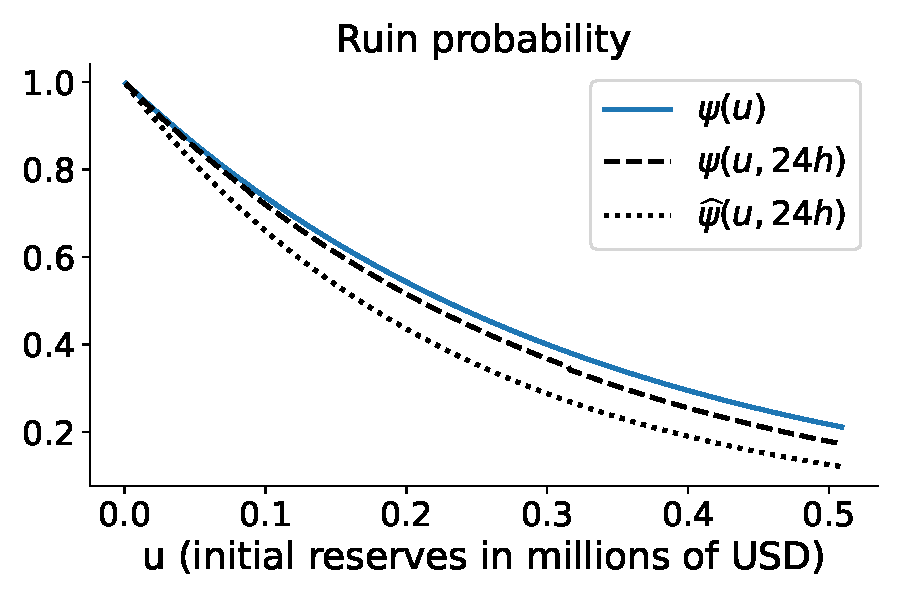
\includegraphics[width=0.45\textwidth]{../Figures/rp_exp_fixed_time}
%       \label{sub:rp_exp_fixed_time}
%                          }
%                          \hskip1em
%     \subfloat[$V(u, t)-u, \widehat{V}(u,t)-u$ and $\mathbb{E}(R_t) - u$.]{
%       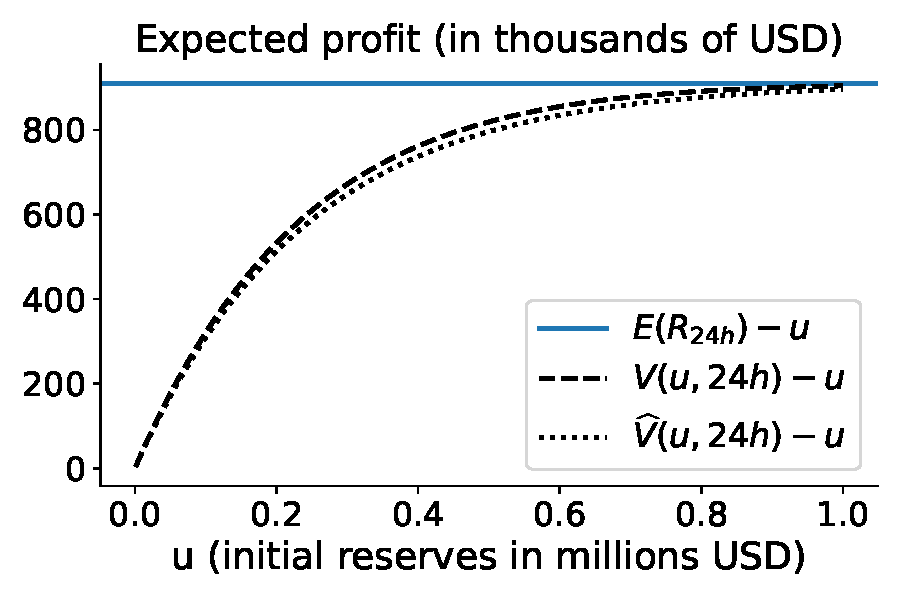
\includegraphics[width=0.45\textwidth]{../Figures/V_exp_fixed_time}
%       \label{sub:V_exp_fixed_time}
%                          }

%     \caption{Ruin probabilities and expected profit given that ruin did not occur.}
%     \label{fig:rp_V_exp_fixed_time}
%   \end{center}
% \end{figure}
% An exponential time horizon tends to put more weight on smaller time horizon, which results in smaller ruin probability \cref{sub:rp_exp_fixed_time} and higher expected profit \cref{sub:V_exp_fixed_time}.
% \end{ex}

% \subsection{Ruin and expected profit of a selfish miner}\label{ssec:selfish_mining}
% Let $(N_t)_{t\geq0}$ be the homogeneous Poisson process with intensity $\lambda$ that governs the block discovery process of the entire network. As in the previous section, we consider a miner named Sam who owns a share $q\in(0,1)$ of the computing power so that a newly found block belongs to Sam with probability $q$.  We keep track of Sam's lead over the honest chain in terms of number of blocks via a Markov jump process
% $$
% X_t=Z_{N_t}, \text{ }t\geq0,
% $$ 
% where $(Z_{k})_{k \geq 0}$ is a homogeneous Markov chain with finite state space $E = \{0,1,0^\ast\}$ which we define now. Consider some time $n\geq0$,
% \begin{itemize}
% \item If Sam is not hiding any block, then $Z_n = 0$, 
% \begin{itemize}
% \item if Sam finds the next block, he stores it in a buffer and $Z_{n+1} = 1$, 
% \item if the other miners discover a block then Sam's buffer remains empty $Z_{n+1}=0$, 
% \end{itemize}
% In both cases, Sam is not collecting any reward.
% \item If Sam is hiding one block at that time, then $Z_n = 1$,
% \begin{itemize} 
% \item if he then finds a new block, then he broadcasts both blocks immediately (which resets the Markov chain to $Z_{n+1}=0$), and he collects two rewards,
% \item if the others find a block, then Sam also releases his block leading to a fork situation characterized by $Z_{n+1} = 0^\ast$. At that moment Sam is not collecting any rewards.
% \end{itemize}
% \item If a fork situation is present at that time ($Z_n = 0^{\ast}$), then 
% \begin{itemize}
% \item if Sam finds a new block then he appends it to his branch of the chain and collects the reward for two blocks and $Z_{n+1} = 0$.  
% \item if the others find a block then 
% \begin{itemize}
% \item they append it to Sam's branch with a probability $0\leq \gamma \leq 1$, in which case Sam gets the reward for one block. 
% \item If the block is mined on top of the competing branch, then Sam earns nothing. 
% \end{itemize}
% In both cases, the number of hidden blocks then becomes $Z_{n+1}=0$.
% \end{itemize}
% \end{itemize}
% Let $(\xi_n)_{n\geq1}$ be a sequence of \iid Bernouill variables with parameter $q$, we have that 
% \begin{equation}\label{eq:gain_function_selfish}
% Z_n = g\left[Z_{n-1},\xi_{n}\right] = \begin{cases}
% 0,&\text{ if } Z_{n-1} =0^\ast,\\
% 0,&\text{ if } Z_{n-1} =1\text{ }\&\text{ }\xi_{n} =1,\\
% 0,&\text{ if } Z_{n-1} =0\text{ }\&\text{ }\xi_{n} =0,\\
% 0^\ast,&\text{ if } Z_{n-1} =1\text{ }\&\text{ }\xi_{n} =0,\\
% 1,&\text{ if } Z_{n-1} =0 \text{ }\&\text{ }\xi_{n} = 1.\\
% \end{cases}
% \end{equation} 
% The process $(Z_n)_{n\geq0}$ is a Markov chain with transition graph provided in \cref{fig:transition_graph}.
% \begin{figure}[!ht]
% \begin{center}
% \begin{tikzpicture}[->, >=stealth', auto, semithick, node distance=3cm]
% \tikzstyle{every state}=[fill=white,draw=black,thick,text=black,scale=0.8]
% \node[state]    (1)                     {$0$};
% \node[state]    (2)[right of=1]         {$1$};
% \node[state]    (3)[above of=2]         {$0^{\ast}$};
% \path
% (1) edge[loop left]     node{$1-q$}        (1)
%     edge[bend left]     node{$q$}          (2)
% (2) edge[bend left]      node{$q$}         (1)
%     edge[bend right]      node{$1-q$}      (3)
% (3) edge[bend right, above]      node{$1$}         (1);
% \end{tikzpicture}
% \end{center}
% \caption{Transition graph of the Markov chain $(Z_k)_{k\geq0}$ representing the stock of blocks retained by Sam when implementing the simplified selfish mining strategy.}
% \label{fig:transition_graph}
% \end{figure} 
% The selfish mining strategy alters the reward collecting process. The surplus process of Sam introduced in \eqref{eq:surplus_protocol} now becomes 
% \begin{equation}\label{eq:surplus_selfish}
% R_t = u-c\cdot t+b\cdot\sum_{n = 1}^{N(t)}f\left[Z_{n-1},\xi_n, \zeta_n\right],
% \end{equation}
% where the $(\xi_n)_{n\ge 1}$ and $(\zeta_n)_{n\ge 1}$ are \iid Bernoulli random variables with parameter $q$ and $\gamma$, respectively, and 
% \begin{equation}\label{eq:gain_function_selfish}
% f\left[Z_{n-1},\xi_n, \zeta_{n}\right] = \begin{cases}
% 0,&\text{ if } Z_{n-1} =0,\\
% 0,&\text{ if } Z_{n-1} =0^\ast\text{ }\&\text{ }\xi_{n} =0\text{ }\&\text{ }\zeta_{n} =0,\\
% 1,&\text{ if } Z_{n-1} =0^\ast\text{ }\&\text{ }\xi_{n} =0\text{ }\&\text{ }\zeta_{n} =1,\\
% 2,&\text{ if } Z_{n-1} =0^\ast\text{ }\&\text{ }\xi_{n} =1,\\
% 2,&\text{ if } Z_{n-1} =1\text{ }\&\text{ }\xi_{n} =1.\\
% \end{cases}
% \end{equation} 
% \noindent It is interesting to see whether selfish mining is still profitable for Sam if the possibility of ruin is included in the analysis. His average earning per time unit is now given by 
% \begin{equation}\label{eq:average_earning_selfish}
% \frac{b}{t}\,\mathbb{E}\left[\sum_{k = 1}^{N_t}f(Z_{k-1},\xi_k,\zeta_k)\right] - c.
% \end{equation}
% This quantity can be determined if we assume that Sam has been mining in a selfish way for quite some time already, so that we can consider the Markov chain to be in stationarity with stationary probabilities
% $$
% \mathbb{P}(Z = 0)=\frac{1}{1+2q-q^2},\text{ }\mathbb{P}(Z = 1)=\frac{q}{1+2q-q^2},\text{ and }\mathbb{P}(Z = 0^{\ast})=\frac{q(1-q)}{1+2q-q^2}.
% $$
% The quantities $U_k:=f\left(Z_{k-1},\xi_k,\zeta_k\right),\text{ }n\geq1$ then have a \pmf $p_U(\cdot): =\mathbb{P}(U = \cdot)$ given by 
% $$
% p_U(0) =\frac{1+q(1-q)+q(1-q)^2(1-q)}{1+2q-q^2},\text{ }p_U(1)=\frac{p\gamma(1-p)^2}{1+2q-q^2},\text{ and }p_U(2)=\frac{q^2+q^2(1-q)}{1+2q-q^2},
% $$
% and the net profit condition correspondingly reads
% \begin{equation*}
% b\lambda\frac{\gamma q(1-q)^2 + 4q^2-2q^3}{1+2q-q^2} - c>0.
% \end{equation*}
% The profitability of selfish mining consequently depends on the interplay between the probabilities $q$ and $\gamma$, and not all values of $q$ and $\gamma$ will lead to positive expected profit. Define 
% \begin{equation*}
% \widehat{\psi}_z(u,t)\equiv \mathbb{E}\left[\psi_z(u,T)\right] = \mathbb{E}\left(\psi(u,T)\Big \rvert Z_0 = z\right)
% \text{ and }\widehat{V}_z(u,t)\equiv \mathbb{E}[V_z(u,T)] = \mathbb{E}\left(R_T\mathbb{I}_{\tau_u>T}\Big \rvert Z_0 = z\right).
% \end{equation*}
% \begin{theo}\label{theo:psi_V_selfish}
% For any $u\ge 0$, the ruin probability and expected profit of a selfish miner are given by
% \begin{equation*}\label{ruin_selfish_app}
% \widehat{\psi}_0(u,t) =
% {\it C_1}\,{{\rm e}^{\rho_1\,u}}+{{\rm e}^{\rho_2\,u}} \left[ {\it C_2}\,
% \cos \left( \rho_3\,u \right) +{\it C_3}\,\sin \left( \rho_3\,u \right)\right],
% \end{equation*}
% and 
% \begin{equation*}
% \widehat{V}_0(u,t)={\it A_1}\,{{\rm e}^{\rho_1\,u}}+{{\rm e}^{\rho_2\,u}} \left[ {\it A_2}\,
% \cos \left( \rho_3\,u \right) +{\it A_3}\,\sin \left( \rho_3\,u \right)\right] +u+C,\label{thisone}
% \end{equation*}
% \end{theo}
% \begin{proof}
% See \citet{Hansjoerg2022}.
% \end{proof}

% The truth is that following the protocol is always more profitable on average, the question is then why selfish mining?\\

% Three reasons:
% \begin{enumerate}
%   \item The relative revenue of selfish miner can be greater than their fair share
%   \begin{itemize}
%     \item It is pivotal when the number of cryptocurrency units that will be issued is bounded. By mining selfishly over the course of the cryptocurrency minting period, the ultimate share of the selfish miner is greater than that of the honest miners.
%   \end{itemize}
%   \item Honest miners waste resources, therefore they might quite making malicious miners more prominent
%   \item Selfish mining slows down the pace of block arrivals leading to a downward adjustment of the cryptopuzzle difficulty
% \end{enumerate}
% Reason 1 is the one invoked in the paper of \citet{Eyal2014}. Reason 2 is probably difficult to study as we would have to model the resilience of honest miners, it probably requires a game theoretic framework. We will try to illustrate numerically reason 3 in \cref{ssec:solo_mining_VS_selfish_mining}.

% \subsection{Solo mining versus selfish mining when including a difficulty adjustment}\label{ssec:solo_mining_VS_selfish_mining}
% Let the time unit be the hour. Since the Bitcoin blockchain protocol is designed to ensure that one block of confirmed transactions is added to the blockchain about every ten minutes, this renders the block arrival intensity in our model to be $\lambda = 6$. The reward $b$ is determined by the number $n_{BTC}$ of bitcoins earned when finding a block and the price $\pi_{BTC}$ of the bitcoin. For the illustrations in this paper, we use the data of January 1, $2020$, when $n_{BTC}=12.5$ and $\pi_{BTC} =\$7,174.74$\footnote{Source:\href{https://www.blockchain.com/}{blockchain.com}}, so that the reward amounts to
% $$
% b = n_{BTC}\times \pi_{BTC} = \$89,684.30.
% $$
% We assume that the operational cost of mining reduces to the electricity consumed when computing hashes. On January 1,  $2020$, the yearly consumption of the network was estimated by the Cambridge Bitcoin Electricity Consumption Index\footnote{Source:\href{https://www.cbeci.org/}{CBEI}} to $72.1671$ TWh.\footnote{The choice of this concrete date for the illustrations in this paper is somewhat arbitrary. Choosing another date and estimate of the Bitcoin price will, however, not crucially change the conclusions as long as the reward for finding a block compensates the operational cost.    
% } We denote by 
% $$
% W = \frac{72.1671\times 10^9}{365.25\times 24}
% $$
% the electricity consumption of the network expressed in kWh. We let the operational cost $c$ of a given miner be proportional to its share $p\in(0,1)$ of the network computing power with 
% $$
% c = p\times W \times \pi_W,
% $$  
% where $\pi_W$ denotes the price of the electricity where the miner is located, expressed in USD per kWh. Mining (at least on the bitcoin blockchain) boils down to drawing random numbers, referred to as hashes uniformly inside the set $\{0,\ldots, 2^{256}-1\}$. The block is mined if the computed hash is smaller than some target $T$. Calibrating $T$ helps to maintain a steady flow of blocks in the blockchain. In the bitcoin blockchain, the target $T$ is set so as to ensure that $6$ blocks are generated per hour. The target may be estimated by comparing $2^{256}$ to the number of hashes computed by the network in ten minutes. On January 1, 2020, the network was computing $97.01$\footnote{Source: \href{https://www.blockchain.com/}{blockchain.com}} exahashes per second. The number of hashes required on average to mine a block is given by the difficulty defined as $D = T_{\max}/T$. Define $H= 97.01 \times 10^{18} \times 3600$ as the number of hashes computed per hour by the network. We then set the target so that $D / H = 6$ which is equivalent to 
% \[
% T = \frac{T_{\max}}{6H}
% \] 
% The difficulty/target is adjusted every $2,016$ blocks by changing the target $T$ to 
% $$
% T^\ast = T\times \frac{t^\ast}{336},
% $$
% where $t^\ast$ is the time (in hours) it took to mine $2,016$ blocks (here $2016/6=336$ hours is the time it should have taken to mine $2,016$ blocks). The difficulty adjustment was studied in \citet{Bowden2020} and led them to conclude that the block arrival process is well captured by a non-homogeneous Poisson process. Following their terminology, we refer to the time elapsed between two difficulty adjustments as a \textit{segment}.\\

% \noindent We now want to quantitatively address whether selfish mining is worthwhile when considering the possibly implied adjustment of the cryptopuzzle difficulty. We do so in a simplified setup, where only Sam may switch between selfish mining and following the protocol, whereas everyone else follows the protocol. Concretely, we compute the ruin probability and expected profit of Sam over two segments when
% \begin{enumerate}
% \item[(i)]  he is following the protocol during both segments,
% \item[(ii)] he applies selfish mining during the first segment and resumes following the protocol during the second segment. 
% \end{enumerate}

% \noindent For (i), we compute the expected profit using the result of \cref{theo:psi_V_T_solo_mining} by setting the average time horizon to $t = 672$ (the number of hours in four weeks). We assume that the arrival intensity of the blocks in the blockchain remains unchanged over the two segments with $\lambda = 6$, as does the cryptopuzzle difficulty $T$.\\

% \noindent For (ii), we proceed as follows. Selfish mining slows down the pace at which the blocks are added to the blockchain, and the number of blocks wasted exactly corresponds to the number of passages of the Markov chain $(Z_n)_{n\geq0}$ through the state $0^\ast$. We know that once stationarity is reached, the probability for  $(Z_n)_{n\geq0}$ to be in state $0^\ast$ is 
% $$
% \frac{q(1-q)}{1+2q-q^2}.
% $$
% We therefore approximate the arrival process in this first segment by a homogeneous Poisson process with intensity 
%  $$
% \lambda_1 = \lambda \times\left(1- \frac{q(1-q)}{ 1+2q-q^2}\right).
% $$ 
% When blocks are being withheld, the average time required to mine $2,016$ blocks increases from $336$ to $t_1 = 2016/\lambda_1$. We hence compute the ruin probability and expected surplus over the first segment using \cref{theo:psi_V_selfish} respectively with time horizon $t_1$. Selfish mining during the first segment then leads to a downward adjustment of the cryptopuzzle difficulty  to $T_2 = T\times{t_1}/{336}$ that will be in force during the second segment. As the miner resumes following the protocol on that second segment, the block arrival process becomes again a proper homogeneous Poisson process with intensity $\lambda_2$ to be determined as follows. Let $H$ be the number of hashes computed per hour (hashrate) by the network. The number of blocks mined per hour is then given by 
% $$
% \lambda_2 = \frac{T_{\max}}{T_2\times H}.
% $$

% The miner's ruin probability and surplus over the second segment are now computed using the formulas of \cref{theo:psi_V_T_solo_mining} using as initial wealth the miner's expected surplus over the first segment
% \[
% u_2 = \widehat{V}_0(u,t), 
% \]
% a block arrival intensity equal to $\lambda_2$ and a reduced time horizon equal to $t_2=2016/\lambda_2$.\\  

% \noindent We consider a miner who owns a share $p = 0.2$ of the network computing power. If he follows the protocol, then the net profit condition holds if $\pi_W<0.065$. If he withholds blocks on the first segment, then the net profit condition frontier depends on the electricity price and the hashpower provided that his connectivity is fixed, for instance set to $q=0.75$. \cref{fig:nbc_segments} shows the net profit condition frontiers for a selfish miner on Segment $1$ who starts following again the protocol on Segment $2$. 
% \begin{figure}[!ht]
%   \begin{center}
%     \subfloat[Net profit condition frontier on Segment 1]{
%       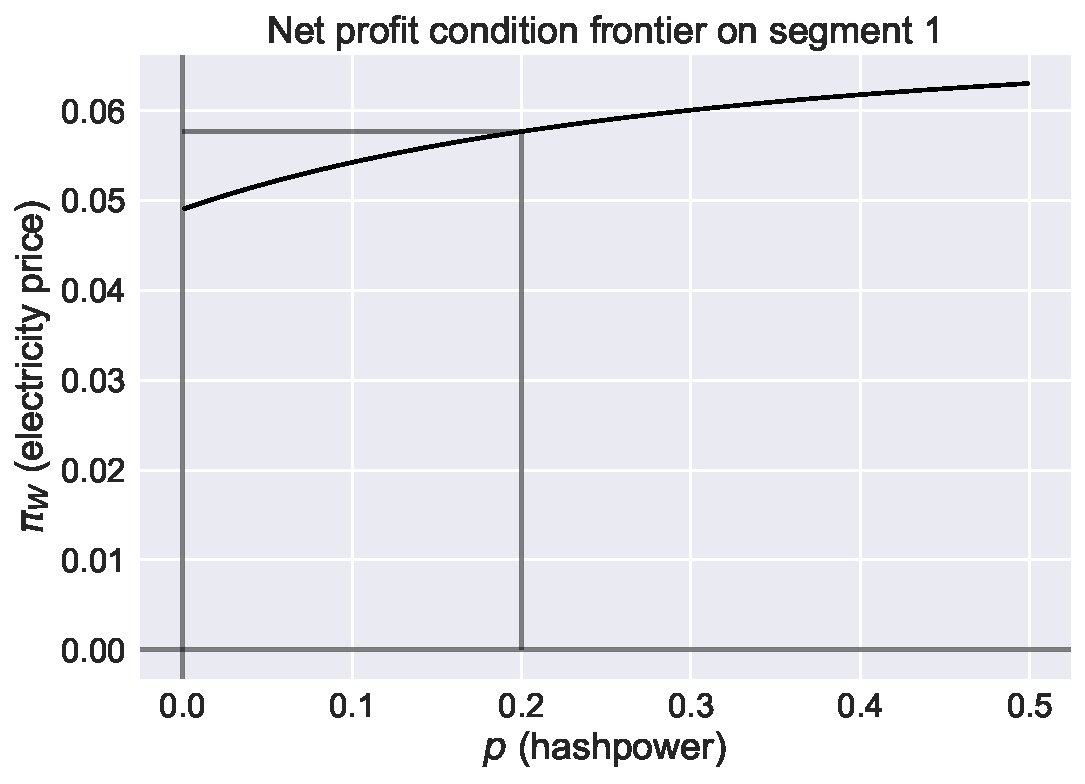
\includegraphics[width=0.45\textwidth]{../Figures/nbc_segment1_12a}
%       \label{sub:nbc_segment1}
%                          }
%                          \hskip1em
%     \subfloat[Net profit condition frontier on Segment 2.]{
%       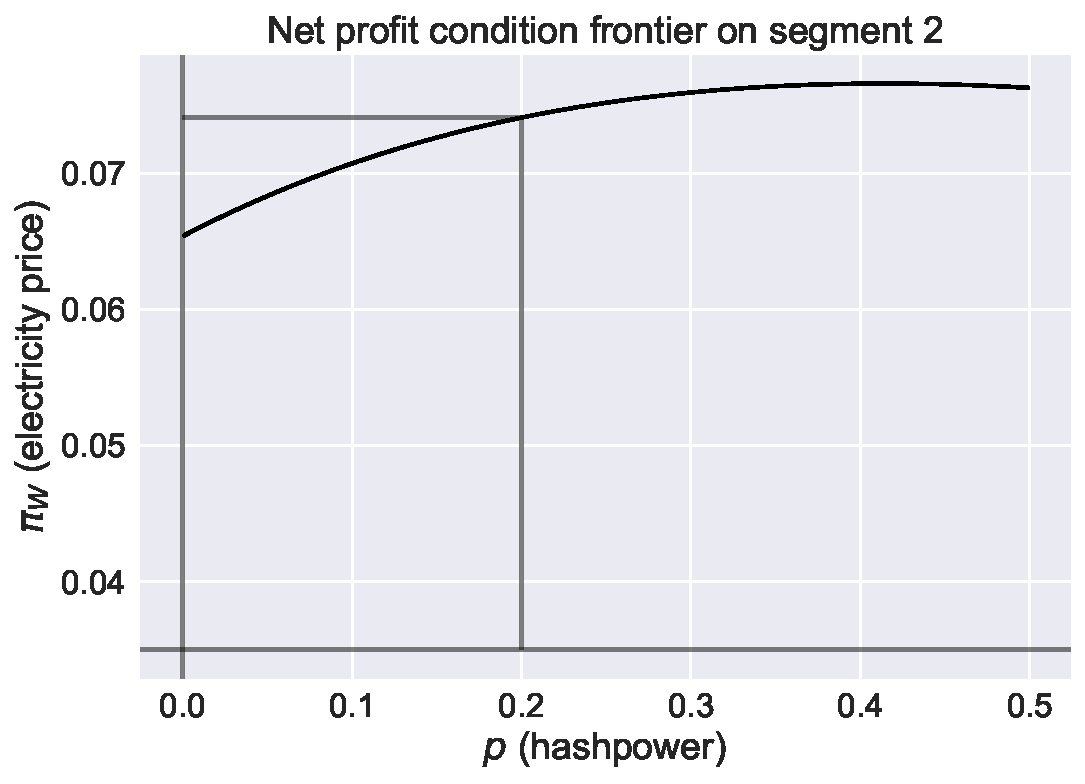
\includegraphics[width=0.45\textwidth]{../Figures/nbc_segment2_12b}
%       \label{sub:nbc_segment2}
%                          }
%     \caption{Net profit condition frontier on Segment 1 and 2 for a selfish miner.}
%     \label{fig:nbc_segments}
%   \end{center}
% \end{figure}
% \noindent In absence of ruin considerations, selfish mining on Segment $1$ is profitable only if the price of electricity is lower than $0.058$, see \cref{sub:nbc_segment1}. Only when the selfish miner owns the totality of the hashpower, is selfish mining as profitable as following the protocol. On Segment $2$, the profitability is always greater than when following the protocol. The profitability on Segment $2$ holds in our case if the electricity price is lower than $0.074$, see \cref{sub:nbc_segment2}. It is interesting to note that by increasing the hashpower beyond a certain threshold we actually lower the profitability during Segment $2$. At higher hashpower levels, the probability of the Markov chain $(Z_n)_{n\geq 0}$ visiting state $0^\ast$ becomes small. In that case fewer blocks are being wasted, which in turn reduces the downward adjustment of the cryptopuzzle difficulty and hence the profitability during Segment 2.\\

% \noindent Figure \ref{fig:rp_difficulty_adjusment} shows the ruin probability of a selfish miner and a miner following the protocol as a function of initial wealth for a range of electricity prices. 
% \begin{figure}[!ht]
%   \begin{center}
%       % \subfloat[$\pi_W = 0.04$.]{
%       % \includegraphics[width=0.45\textwidth]{Figures/rp_difficulty_adjusment_4}
%       % \label{sub:rp_difficulty_adjusment_4}
%       %                    }
%                          \hskip1em
%     \subfloat[$\pi_W = 0.05$.]{
%       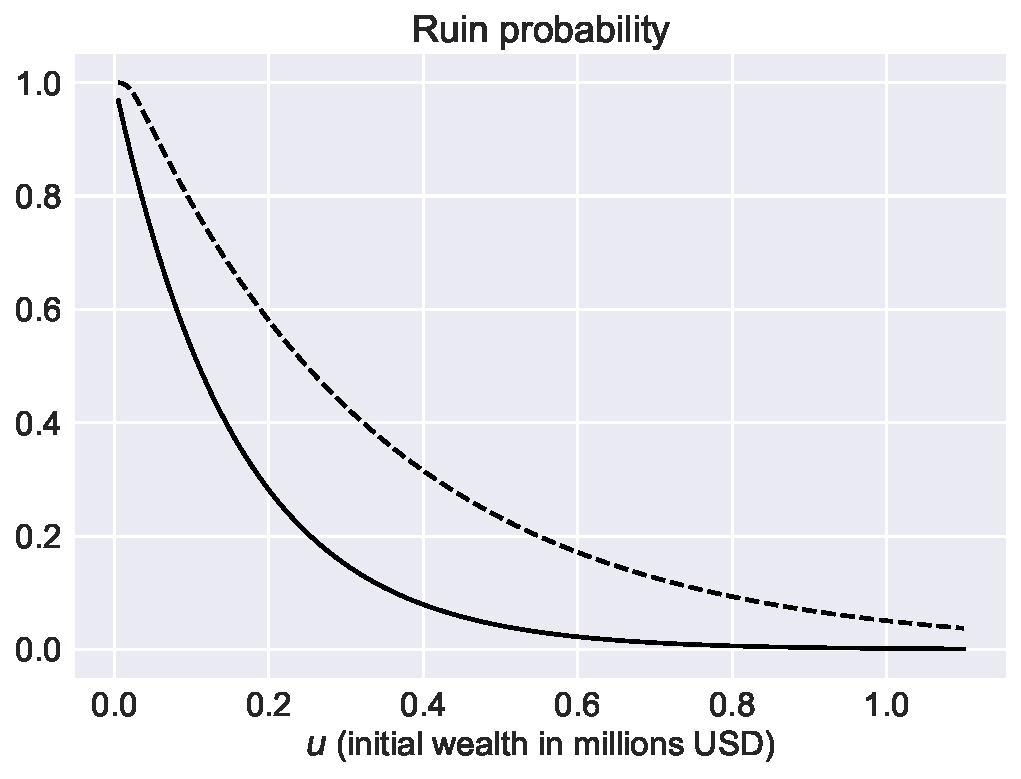
\includegraphics[width=0.45\textwidth]{../Figures/rp_difficulty_adjusment_5_13a}
%       \label{sub:rp_difficulty_adjusment_5}
%                          }
%                          \hskip1em
%        \subfloat[$\pi_W = 0.06$.]{
%       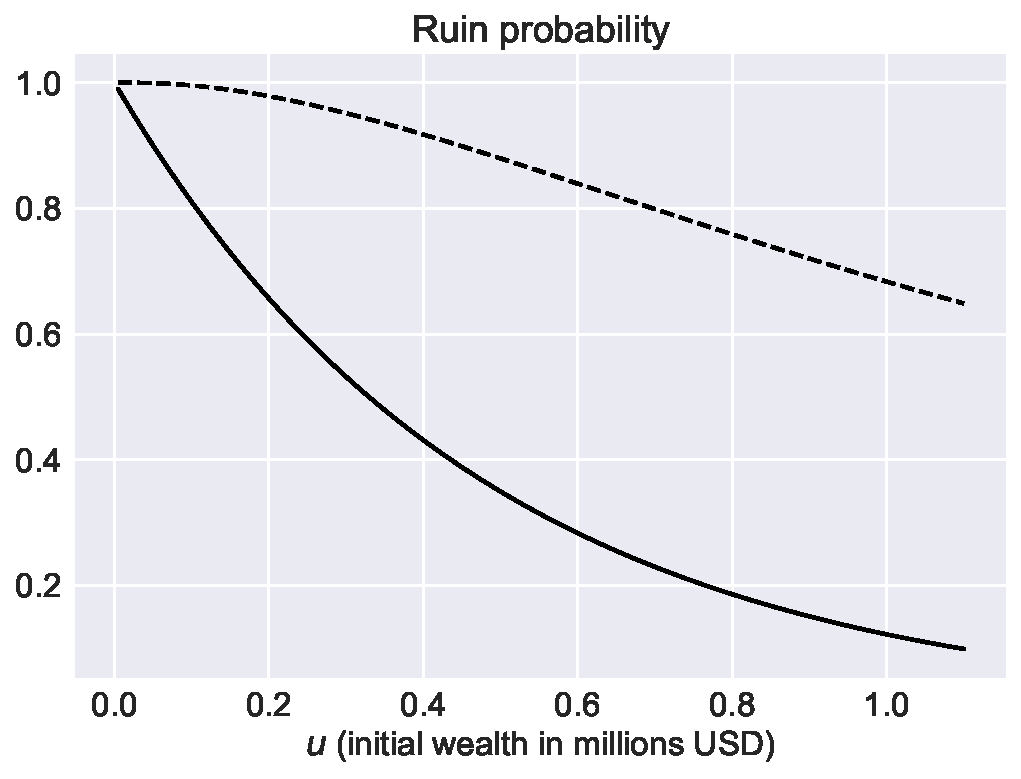
\includegraphics[width=0.45\textwidth]{../Figures/rp_difficulty_adjusment_6_13b}
%       \label{sub:rp_difficulty_adjusment_6}
%                          }
%                          \hskip1em
%     \subfloat[$\pi_W = 0.07$.]{
%       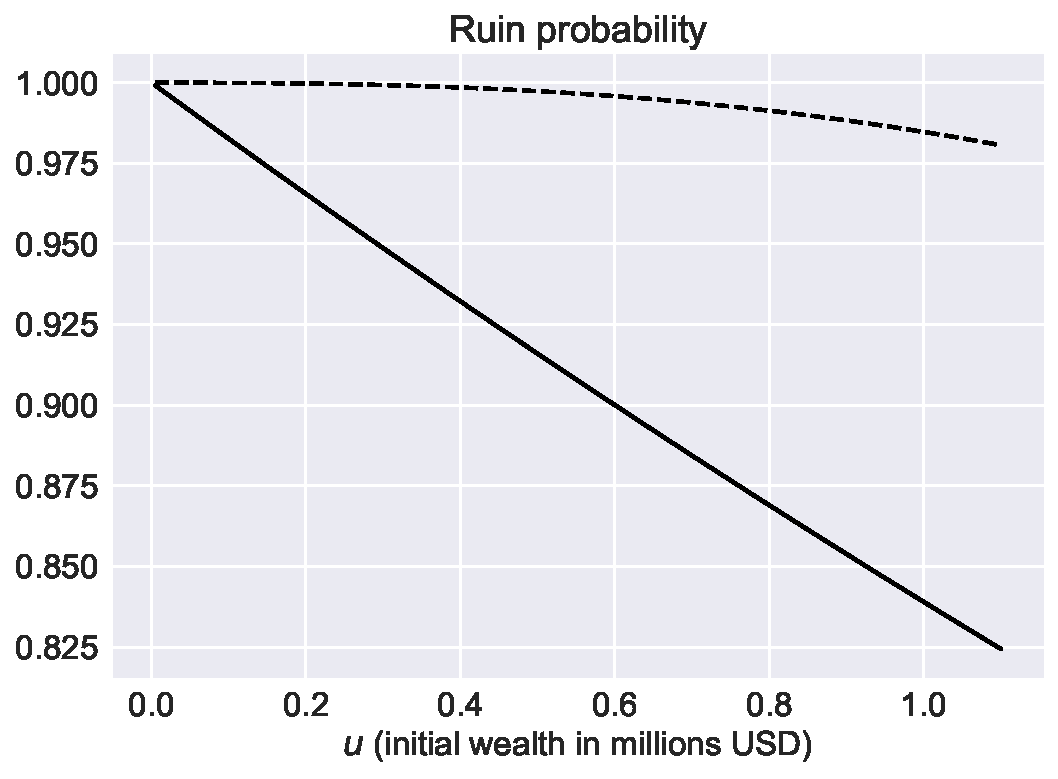
\includegraphics[width=0.45\textwidth]{../Figures/rp_difficulty_adjusment_7_13c}
%       \label{sub:rp_difficulty_adjusment_7}
%                          }
%                          \hskip1em
%        \subfloat[$\pi_W = 0.08$.]{
%       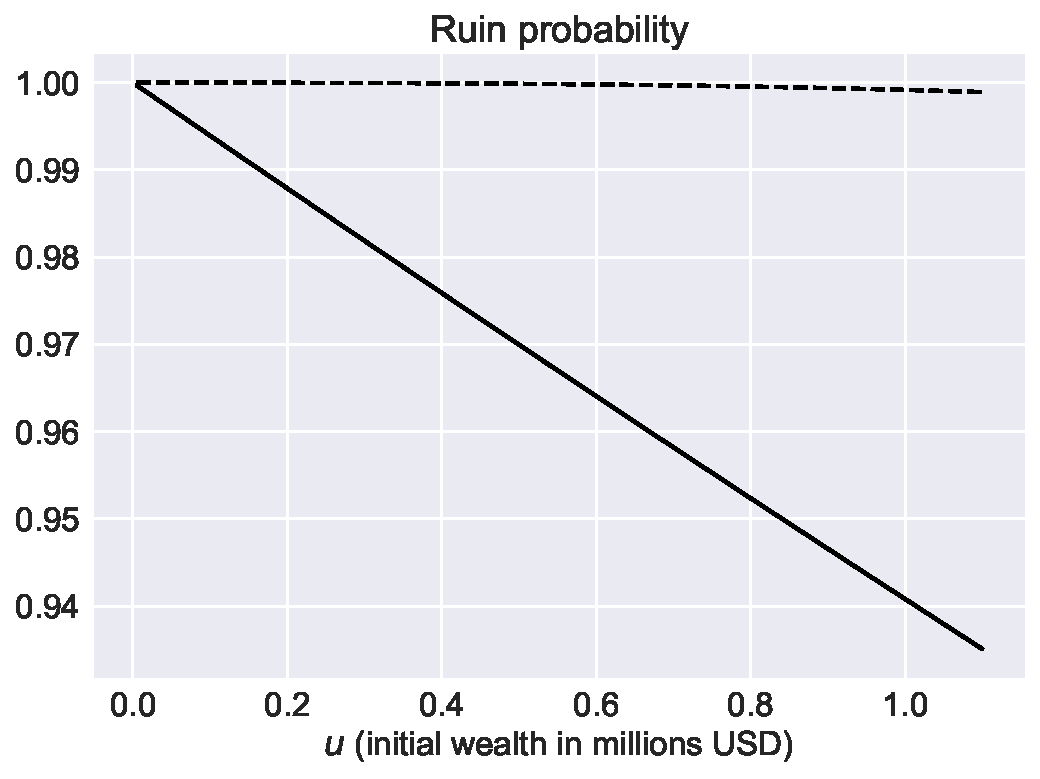
\includegraphics[width=0.45\textwidth]{../Figures/rp_difficulty_adjusment_8_13d}
%       \label{sub:rp_difficulty_adjusment_8}
%                          }
%                          \hskip1em
%     % \subfloat[$\pi_W = 0.09$.]{
%     %   \includegraphics[width=0.45\textwidth]{../Figures/rp_difficulty_adjusment_9}
%     %   \label{sub:rp_difficulty_adjusment_9}
%     %                      }
%     \caption{Ruin probability over two segments as a function of initial wealth of a miner following the protocol (solid) and a selfish miner (dashed) for various electricity prices with hashpower $p=0.2$ and connectivity $q=0.75$.}
%     \label{fig:rp_difficulty_adjusment}
%   \end{center}
% \end{figure}
% From a ruin probability perspective, reducing the difficulty adjustment does not compensate for the risk involved in implementing selfish mining. 

% Figure \ref{fig:rev_difficulty_adjusment} displays the expected profit of a selfish miner and a miner following the protocol as a function of initial wealth for a range of electricity prices.
% \begin{figure}[!ht]
%   \begin{center}
%       % \subfloat[$\pi_W = 0.04$.]{
%       % \includegraphics[width=0.45\textwidth]{../Figures/rev_difficulty_adjusment_4}
%       % \label{sub:rev_difficulty_adjusment_4}
%       %                    }
%                          \hskip1em
%     \subfloat[$\pi_W = 0.05$.]{
%       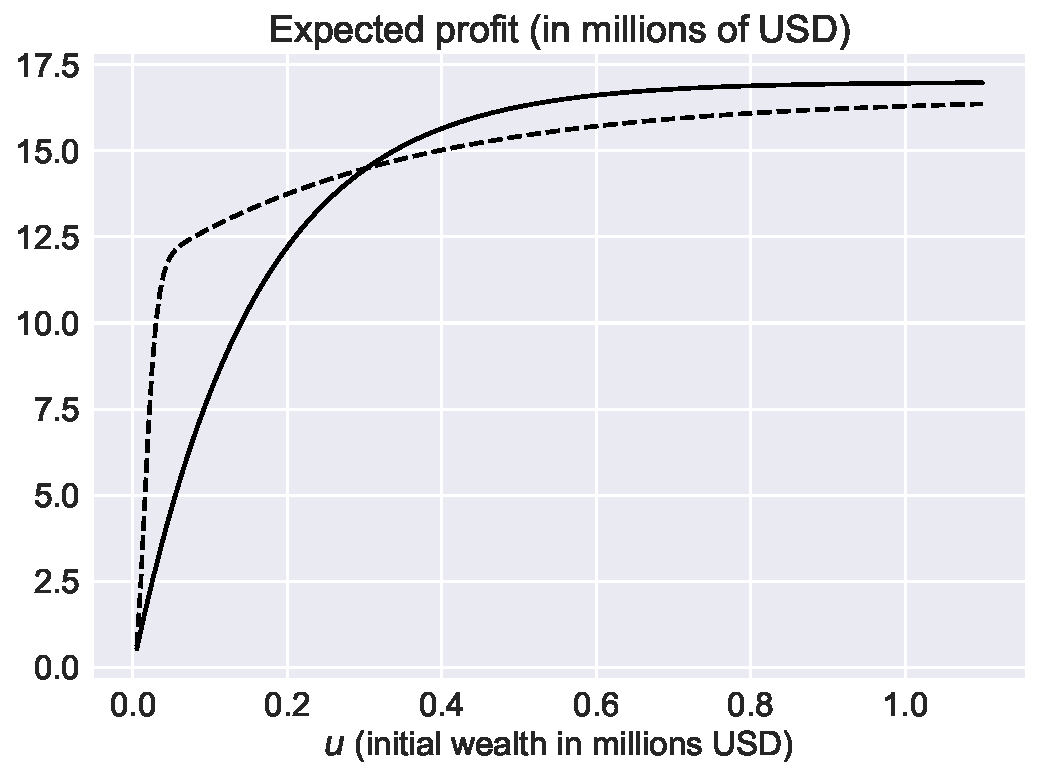
\includegraphics[width=0.45\textwidth]{../Figures/rev_difficulty_adjusment_5_14a}
%       \label{sub:rev_difficulty_adjusment_5}
%                          }
%                          \hskip1em
%        \subfloat[$\pi_W = 0.06$.]{
%       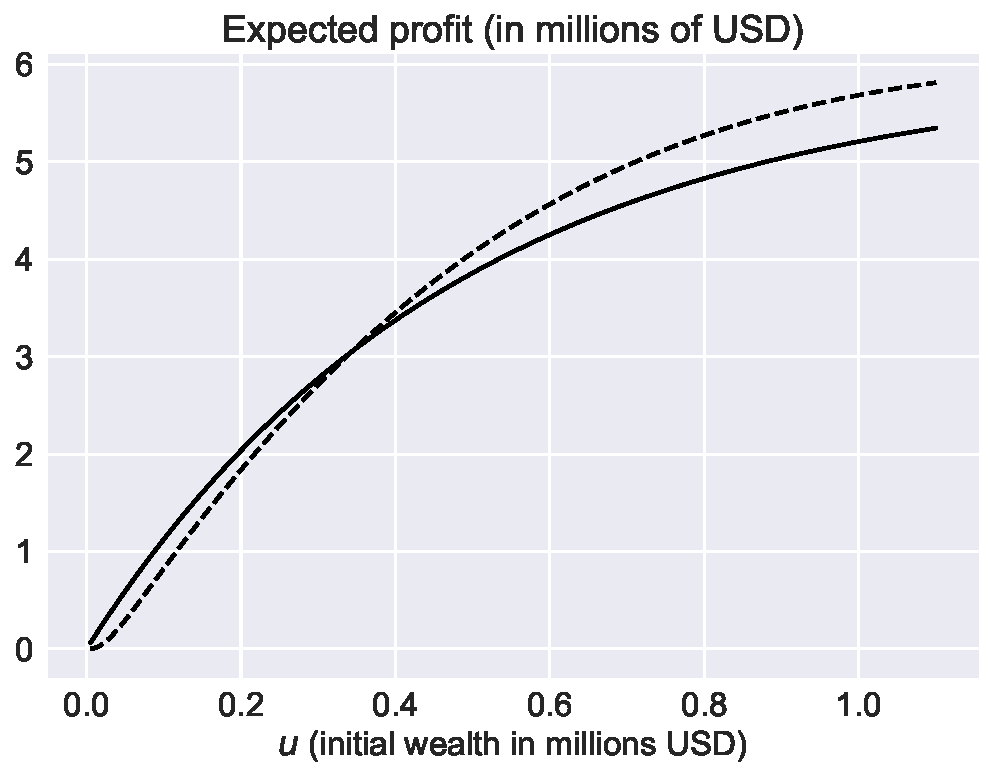
\includegraphics[width=0.45\textwidth]{../Figures/rev_difficulty_adjusment_6_14b}
%       \label{sub:rev_difficulty_adjusment_6}
%                          }
%                          \hskip1em
%     \subfloat[$\pi_W = 0.07$.]{
%       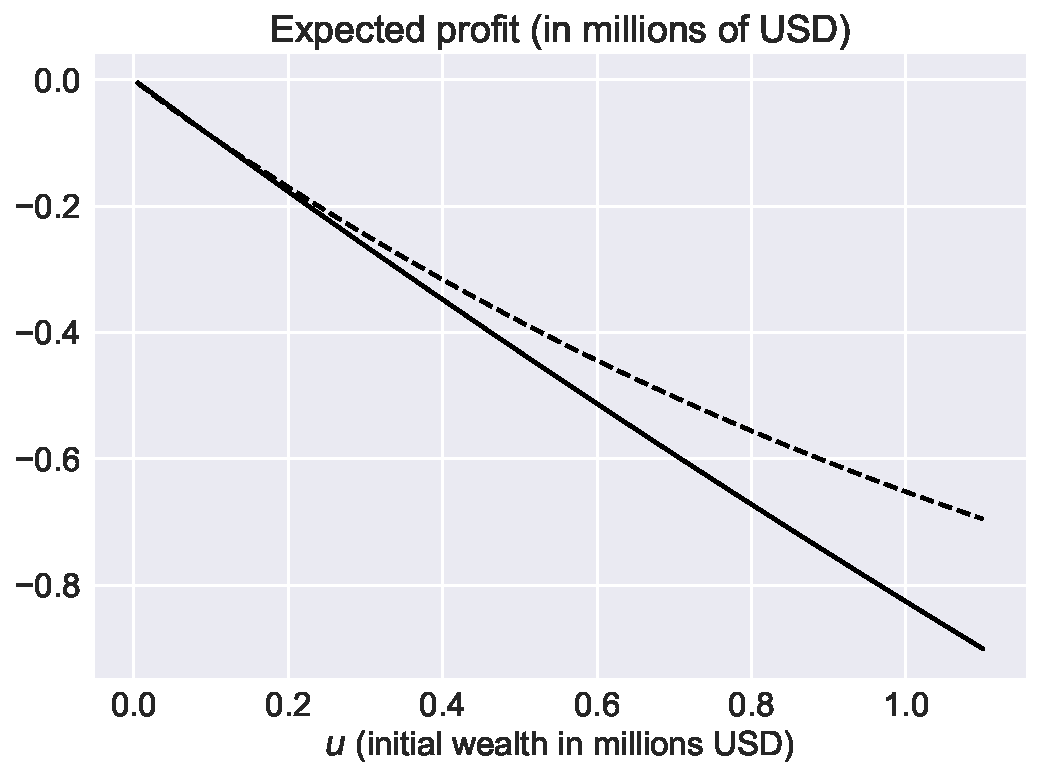
\includegraphics[width=0.45\textwidth]{../Figures/rev_difficulty_adjusment_7_14c}
%       \label{sub:rev_difficulty_adjusment_7}
%                          }
%                          \hskip1em
%        \subfloat[$\pi_W = 0.08$.]{
%       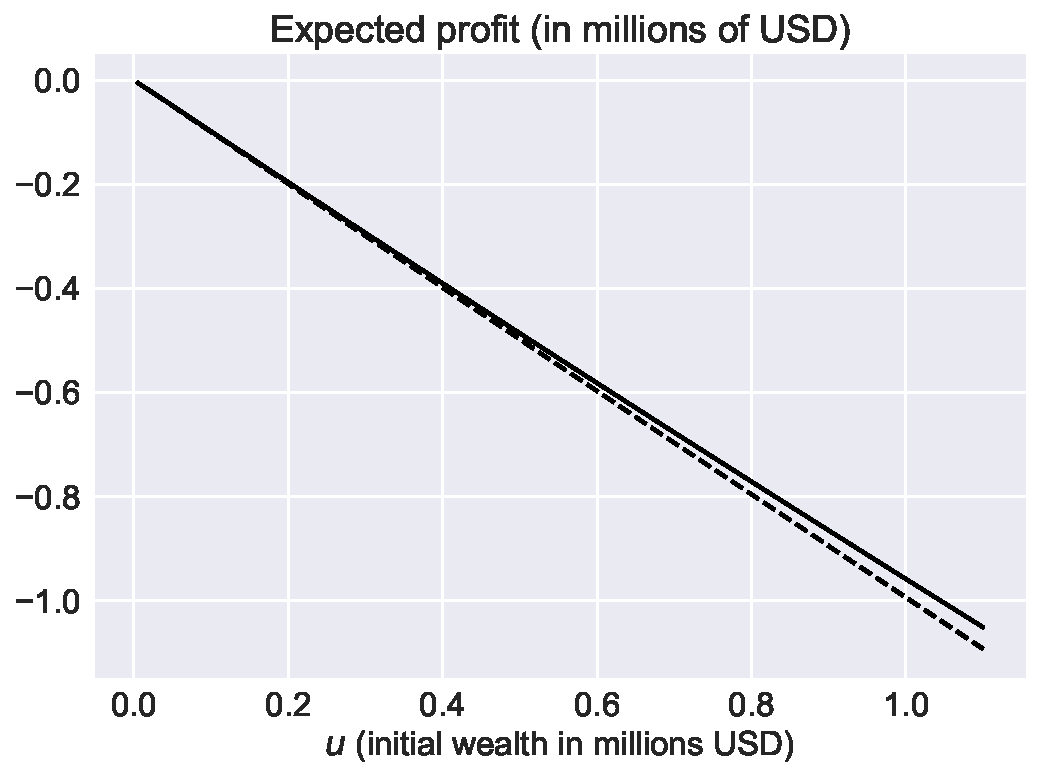
\includegraphics[width=0.45\textwidth]{../Figures/rev_difficulty_adjusment_8_14d}
%       \label{sub:rev_difficulty_adjusment_8}
%                          }
%                          \hskip1em
%     % \subfloat[$\pi_W = 0.09$.]{
%     %   \includegraphics[width=0.45\textwidth]{../Figures/rev_difficulty_adjusment_9}
%     %   \label{sub:rev_difficulty_adjusment_9}
%     %                      }
%     \caption{Expected profit over two segments as a function of initial wealth of a miner following the protocol (solid) and a selfish miner (dashed) for various electricity prices with hashpower $p=0.2$ and connectivity $q=0.75$.}
%     \label{fig:rev_difficulty_adjusment}
%   \end{center}
% \end{figure}
%  One can observe the different profit and loss profile of a selfish miner compared to that of a miner following the protocol on both segments. If the net profit condition holds when following the protocol, then it also holds for the second segment when blocks were withheld during the first segment. For electricity prices $\pi_W = 0.05, 0.06$, the expected profit as a function of $u$ reaches a plateau of level 
% \begin{equation}\label{eq:plateau_protocol}
% (c-b\lambda q)\times t
% \end{equation}
% when following the protocol, and 
% \begin{equation}\label{eq:plateau_selfish}
% (c-b\lambda_2 q)\times t_2,
% \end{equation}
% when selfish mining is applied during the first segment.  For $\pi_W = 0.05$, the plateau when following the protocol \eqref{eq:plateau_protocol} is higher than the plateau when withholding blocks \eqref{eq:plateau_selfish}, but the expected profit at lower initial wealth is greater for the selfish miner, see Figure \ref{sub:rev_difficulty_adjusment_5}. The exact opposite holds when $\pi_W = 0.06$, see Figure \ref{sub:rev_difficulty_adjusment_6}. The latter is probably the most desirable situation for a selfish miner. For $\pi_W = 0.07$, the net profit condition no longer holds when following the protocol which entails a loss, it holds however on the second segment of the selfish miner but it does not compensate for the loss incurred during the first segment, see Figure \ref{sub:rev_difficulty_adjusment_7}. Selfish mining helps at least in slightly mitigating the losses in this case. For electricity prices $\pi_W > 0.074$, the net profit condition breaks down in each case, resulting in huge losses for both the selfish and the honest miner (cf.\ Figure \ref{sub:rev_difficulty_adjusment_8} ).\\


% \noindent The above analysis allowed us to distinguish situations where selfish mining can be considered worthwile and when it may not. In particular, it turns out that selfish mining can be advisable when following the protocol is not profitable. 

% % \section{Nothing-at-stake in PoS}\label{sec:NaS}
% % \newpage